\documentclass[12pt,a4paper]{article}

% Seitengestaltung
\usepackage[left=3cm,right=2cm,top=2.5cm,bottom=1.5cm,includeheadfoot]{geometry}

% Anpassung von LaTeX an die deutsche Sprache
\usepackage[english, ngerman]{babel}
 
% Mathematik
\usepackage{amsmath}

% Grafiken und Bilder
\usepackage{graphicx}
\graphicspath{ {resources/} }
% Schriftfarbe
\usepackage{xcolor}

% Indexerstellung
\usepackage{makeidx}

% Blindtext
\usepackage{blindtext}
\usepackage{lipsum}

% Umlaute
\usepackage[utf8]{inputenc}

% Zitate an Sprache angepasst
\usepackage{csquotes}

% Verbesserte Schrift
\usepackage{microtype}

% Verlinkungen
\usepackage{hyperref}

% Bessere Tabellen
\usepackage{array}
%\usepackage[table]{xcolor}

% Zeichensatz
\usepackage[T1]{fontenc}

% Schriftart
\usepackage{lmodern}

% Figure a b
\usepackage{subcaption}

% Code Highlighting
\usepackage{listings}

% Acronyme und Glossar
\usepackage[acronym, toc]{glossaries}

% Literaturverzeichniss
\usepackage[backend=bibtex,style=authoryear]{biblatex}

\addbibresource{main.bib}
\makeglossaries
\newglossaryentry{benchmark}
{
  name=benchmark,
  description={Ein Benchmark im Software Performance Testing ist
      eine Metrik oder ein Bezugspunkt, mit dem Softwareprodukte oder -dienstleistungen verglichen werden können, um deren Qualität zu bewerten.
      Beliebte Benchmarks sind beispielsweise CPU-Auslastung, Speicherverbrauch, Durchsatz, Startzeiten aber auch Fehlerrate und Fehlertoleranz.
    }
}
\newglossaryentry{latenz}
{
  name=latenz,
  description={
      Die Latenz ist ein Maß dafür, wie schnell ein Server auf Anfragen des Clients reagiert.
      Die Latenz wird normalerweise in Millisekunden (ms) gemessen und wird oft als Antwortzeit bezeichnet.
      Niedrigere Zahlen bedeuten schnellere Antworten. Die Latenz wird clientseitig gemessen, von der
      Zeit, zu der die Anfrage gesendet wird, bis die Antwort eingeht. Netzwerk-Overhead ist in dieser Zahl enthalten.}
}
\newglossaryentry{durchsatz}
{
  name=durchsatz,
  description={Der Durchsatz gibt an wieviele Anfragen während eines spezifischen Zeit Intervalls von einem Server verarbeitet werden konnen.
      Der Durchsatz wird normalerweise in Anfragen pro Sekunde (requests/sec) angegeben.}
}

\newglossaryentry{perzentile}
{
  name=perzentile,
  description=
    {In der Statistik ist ein Perzentil (oder ein Zentil) ein Wert, unter den ein bestimmter Prozentsatz von Werten in seiner Häufigkeitsverteilung fällt.
      Wenn die Antwortzeit im 50. Perzentil 100ms beträgt, bedeutet dies, dass 50\% der Anfragen in 100ms oder weniger zurückgegeben wurden.
    }
}

\newglossaryentry{hdrHistogramm}{
  name=hdrHistogramm,
  description={Histogramme die das Aufnehmen und Analysieren von
      ausgewählten Daten über eine konfigurierbare, ganzzahlige Reichweite und eine konfigurierbare
      Genauigkeit innerhalb dieser Reichweite ermöglichen \parencite{HdrHistogramm}
      TODO: Add JavaEE APIS jax rs, orm, json, publisher, subscriber, IO Operationen, SPA, Servlet-Container,
      callback (The answer is that you instead pass a callback[7]
      (a lambda) to f as an additional argument, and the body of f spawns a task that calls this lambda with the result when it’s ready)
    },
  user1={hdrHistogramme}
}
\newacronym{http}{HTTP}{Hypertext Transfer Protocol}
\newacronym{hdrhistogram}{HdrHistogramm}{High dynamic range histogram}
\newacronym{cpu}{CPU}{Central processing unit}
\newacronym{ram}{RAM}{Random-access memory}
\newacronym{spa}{SPA}{Single page application}

% !TEX root = main.tex
\hypersetup{
	pdftitle={Master-Arbeit},
	pdfsubject={Reactive Programming mit Quarkus},
	pdfauthor={Erik Simonsen},
	pdfkeywords={Reactive, Reactive Programming, Quarkus, Java},
	pdfstartpage={1},
	plainpages=false,
	hypertexnames=false
}

% !TEX root = main.tex
\usepackage{ntheorem}
\usepackage{mdframed}

\theoremstyle{break}
\theoremheaderfont{\bfseries}
\newmdtheoremenv[
nobreak=true,
linecolor=red,
linewidth=2,
leftmargin=0,
rightmargin=0,
backgroundcolor=yellow,
innertopmargin=10pt,
ntheorem]{todo}{TODO}[section]

\begin{document}
\begin{minipage}{2.1cm}
	
\includegraphics[width=2cm]{resources/fh_logo_klein.jpg}
\end{minipage}
\begin{minipage}{10.0cm}
	Ostfalia - Hochschule für angewandte Wissenschaften\\
	Fakultät Informatik\\
	Institut für Software Engineering
\end{minipage}

\vspace{35mm}

\begin{center}
	{\LARGE Master-Arbeit}
	\\[10mm]
\end{center}

\begin{center}
	\LARGE \textbf{Reactive Programming mit Quarkus\\[28mm]}
\end{center}

\begin{table}[h]
	\centering
	\hspace{50mm}\begin{tabular}{lcll}
		eingereicht von &  & Erik Simonsen           & 70455429 \\

		Erstprüfer:     &  & Prof. Dr. B. Müller     &          \\
		Zweitprüfer:    &  & Prof. Dr. H. Grönninger &          \\
	\end{tabular}
\end{table}

\vspace{30mm}

\begin{table}[h]
	\begin{tabular}{lll}
		Wolfenbüttel, den \today \\
	\end{tabular}
\end{table}
\clearpage

\begin{abstract}
    \normalsize
    \noindent
    Das Ziel der vorliegenden Masterarbeit ist es, das Konzept von reaktiver Programmierung und reaktiven Systemen,
    speziell im Java Ökosystem, zu erläutern. Zudem wird untersucht, ob eine reaktive Anwendung nach dem \verb|Reactor Pattern| das, durch
    Threadwechsel bedingte, Skalierungsproblem einer nicht-reaktiven, auf dem \verb|Thread per request|-Pattern basierenden,
    Anwendung bei hohen Lasten lösen kann.\newline

    Dafür wurden in einem Versuchsaufbau eine Reihe von Lasttests mit stetig steigenden Lasten, jeweils mit und ohne Datenbankanbindung,
    an zwei konzeptionellen Anwendungen,
    reaktiv und nicht-reaktiv, durchgeführt. Dabei wurden leistungsrelevante Metriken wie Durchsatz, Speicherbedarf und CPU-Auslastung gemessen.
    Anschließend wurden die Ergebnisse beider Anwendungen ausgewertet und miteinander verglichen.
    Beide Anwendungen wurden dabei mit dem Full-Stack, Kubernetes-nativen Java-Anwendungsframework \verb|Quarkus| implementiert.\newline

    Die Auswertung der Messergebnisse zeigt, dass die reaktive Anwendung sowohl beim Arbeiten mit statischen, als auch dynamischen Daten
    mit Datenbankanbindung in jeder gemessenen Metrik, besonders im Durchsatz, der nicht-reaktiven Anwendung überlegen ist.
    Bezüglich der Verständlichkeit, Wartbarkeit und Integrationsfähigkeit ist sie nach Auffassung des Autors gegenüber
    einer nicht-reaktiven, traditionellen Anwendung jedoch im Nachteil.
    Die Testergebnisse sind außerdem durch eine Vielzahl
    an Faktoren, wie Hardwareleistung oder Datenbankgröße, beeinflussbar, weswegen der Autor empfiehlt die Testumgebung
    an die eigenen Anforderungen anzupassen.
    Darüber hinaus werden Alternativen zum reaktiven Modell im Java-Umfeld dargestellt und bewertet.\newline

    Weiterführende Arbeiten in diesem Bereich könnten die genannten Metriken von alternativen Ansätzen, wie der Nutzung von virtuellen Threads durch Project Loom,
    in einem ähnlichen Versuchsaufbau untersuchen und mit einer reaktiven Anwendung vergleichen.
\end{abstract}

\clearpage
\thispagestyle{empty}

\section*{Ehrenwörtliche Erklärung}

Hiermit erkläre ich ehrenwörtlich, dass ich die vorliegende Arbeit selbstständig und ohne unerlaubte fremde Hilfe angefertigt habe, andere als die angegebenen Quellen nicht benutzt und die  benutzten Quellen wörtlich oder die inhaltlich entnommenen Stellen als solche kenntlich gemacht habe.
\vspace{4em}\\
Wolfenbüttel, den \today

\tableofcontents
% Verzeichnis von Abbildungen
\listoffigures
% Verzeichnis von Listings
\lstlistoflistings
% Verzeichnis von Tabellen
\listoftables

\setcounter{page}{1}
\pagenumbering{arabic}
\pagestyle{headings}

\section{Einleitung}
\label{sec:einleitung}
In der folgenden Arbeit sind die ersten Vorkommen von möglicherweise nicht geläufigen Begriffen und Abkürzungen, die
im Fließtext nicht erklärt werden, mit einem \verb|(*)| gekennzeichnet.
Diese Begriffe werden im Glossar und/oder Akronymverzeichnis kurz erklärt.

\subsection{Problemstellung}
\label{subsec:problemstellung}
In den letzten Jahren sind die Anforderungen an Webanwendungen durch zunehmende Digitalisierung und entsprechend steigenden Nutzerzahlen,
sowie stark auf Client-Server Kommunikation basierenden Architekturen, wie Microservices und \Glspl{spag}(*), erheblich gestiegen.

Während geschäftskritische Anwendungen lange Zeit mit ein paar Tausend Anfragen pro Sekunde als hoch frequentiert
galten, müssen solche Webanwendungen heutzutage in der Lage sein eine vielfach höhere Last bewältigen zu können.
Darüber hinaus müssen sie \verb|skalierbar| sein, also ohne Leistungseinbußen auf variable Lasten reagieren können.

Das Standardmodell für Java-basierte Webanwendungen ist das \verb|Thread per request|-Modell.
Dabei wird jede HTTP-Anfrage an einen Kernel-Thread gebunden, welcher anschließend die Anfrage sequentiell abarbeitet.
Damit eine möglichst hohe Anzahl an Anfragen parallel abgearbeitet werden kann, wird jedem Thread nur ein Teil der verfügbaren
CPU-Rechenzeit eines CPU-Kerns zugewiesen. Sobald die Rechenzeit eines Threads abgelaufen ist, oder er durch einen blockierenden
Funktionsaufruf in einen inaktiven Zustand versetzt wird, wird der nächste Thread bearbeitet: es erfolgt ein \verb|Threadwechsel|.

Obwohl Threadwechsel, im Gegensatz zu Prozesswechseln, sehr kostengünstig sind, sind sie in diesem Modell ab einer kritischen Anzahl von HTTP-Anfragen
pro Sekunde der begrenzende Skalierungsfaktor. Die Threadwechsel zwischen den Kernel-Threads des Betriebssystems erfolgen dann nicht mehr
schnell genug um jede Anfrage bzw. jeden Thread innerhalb einer akzeptablen Zeit zu bearbeiten.
Diese Begrenzung äußert sich letztendlich darin, dass der \Gls{durchsatz}(*) der Anwendung nicht ausreichend skaliert.

\subsection{Ziel der Arbeit}
\label{subsec:ziel}
Um höhere Workloads zu bewältigen und Anwendungen skalierbarer zu machen, existieren alternative
Anwendungsmodelle, wie das in dieser Arbeit thematisierte \verb|Reactor-Pattern|.
Das Modell nutzt einen Thread pro CPU-Kern und verzichtet somit auf anwendungsbedingte Threadwechsel.
Die Voraussetzung dafür ist allerdings, dass die vorhandenen Threads niemals in einen inaktiven Zustand geraten.
Deswegen dürfen Anfragen an externe Komponenten, wie Datenbanken oder Webservices, den Thread nicht blockieren,
und der vom Ergebnis abhängige Code muss reaktiv, also erst beim tatsächlichen Eintreffen der Antwort,
ausgeführt werden: man spricht von \verb|reaktiver Programmierung|.
Reaktive Programmierung erfordert, dass die Programmlogik jeder
Anwendungsschicht asynchron und eventbasiert strukturiert wird.
Nachdem eine Anfrage an eine externe Komponente abgesetzt wurde, beginnt der Thread bereits mit der Abarbeitung der nächsten
HTTP-Anfrage. Sobald ein Resultat verfügbar ist, wird es dem Thread mithilfe eines Events mitgeteilt.
Dieser führt daraufhin den, für dieses Event hinterlegten, Code aus. Durch diese grundlegende Funktionsweise wird auf anwendungsbedingte
Threadwechsel verzichtet.

In dieser Arbeit wird untersucht, ob \verb|Reactive Programming| bzw. reaktive Anwendungen das Problem der Skalierbarkeit
für hohe Lasten praktikabel lösen können und welche alternativen Lösungsansätze es gibt.

\subsection{Vorgehensweise}
\label{subsec:vorgehensweise}
Um das Verhalten der beiden Modelle unter Last zu prüfen und miteinander zu vergleichen, werden zwei triviale Anwendungen implementiert,
reaktiv und nicht-reaktiv, und einer Reihe von Lasttests mit unterschiedlichen \verb|workloads| unterzogen.
Dabei werden verschiedene \Glsplural{benchmark}(*), wie Durchsatz, Speicherbedarf und CPU-Auslastung gemessen.
Die Anwendungen werden sowohl auf der \acrshort{jvm}(*), als auch nativ ausgeführt und jeweils mit und ohne Datenbankenanbindung getestet.

\subsection{Aufbau}
\label{subsec:aufbau}
Zu Beginn der Arbeit werden in Kapitel \ref{sec:grundlagen} die Grundlagen der Thematik erläutert. Diese beinhalten
Kernel- und User-Threads, blockierende und nicht-blockierende Ein-/Ausgabe-Operationen sowie die beiden darauf aufbauenden Design-Patterns
\verb|Thread per request| und \verb|Reactor|.

Anschließend wird in Kapitel \ref{section:reaktive_programmierung} die Funktionsweise von \verb|Reactive Programming|, und dessen
zugrundeliegendes Konzept von reaktiven Datenströmen erläutert. Danach werden die Vor- und Nachteile des Programmierparadigmas
genannt.
Darauffolgend werden die Eigenschaften von reaktiven Systemen und deren Beziehung untereinander beschrieben.
Zum Ende des Kapitels wird auf die Unterstützung für reaktive Anwendungen und Architekturen innerhalb des Java Ökosystem
sowie Alternativen eingegangen.

In Kapitel \ref{section:vergleich_reaktiv_blockierend} wird zuerst die Testumgebung definiert sowie Testaufbau und Testablauf beschrieben.
Im Anschluss werden die Testresultate genannt und in Form von Diagrammen dargestellt.
Abschließend erfolgt die Auswertung und Erläuterung der Testresultate.
\newpage
% Definiere Style für Text Listings.
\lstdefinestyle{text}{
    basicstyle=\ttfamily\footnotesize
}
% Verwende Style 
\lstset{style=text}
% !TEX root = main.tex

\section{Grundlagen}
\label{section:grundlagen}

\subsection{Threads \& Prozesse in Java}
\label{sections:treads_prozesse}
In der Java-Laufzeitumgebung sind Prozesse und Threads als Betriebssystem-Prozesse realisiert, sog. \textit{native threads} oder auch \textit{Kernelthreads}.
Hierbei wird die Ausführungsreihenfolge, die Ausführungszeit und der Prozess- \& Threadwechsel
vom Scheduler \& Dispatcher des Betriebssystems übernommen \parencite{Tanenbaum2016}.
Die Threading-Abstraktion in Java bietet Entwicklern verhältnismäßig leichten Zugriff auf parallelle Programmierung und Synchronisation von Threads.\newline
Servlet-Container binden üblicherweise jede vom Webserver weitergeleitete Anfrage an einen
Thread\footnote{Aus einem, im vornherein erzeugten, Thread-Pool} im Servlet-API, welcher die jeweilige Anfrage imperativ abarbeitet
(daher auch \textit{worker thread}).\newline
Der auszuführende Code ist in diesem Ansatz an den jeweiligen Thread gekoppelt, dieser wartet bei
asynchronen Ereignissen solange, bis er eine Antwort erhält und blockiert den Thread bis dahin.

Um jede Anfrage, und somit jeden Thread, scheinbar parallel zu bearbeiten wird vom Scheduler
des Betriebssystems regelmäßig ein Kontextwechsel zwischen den Threads,
ein \textit{thread-switch}, durchgeführt. Während bei einem Prozesswechsel der gesamte Programmkontext (Adressraum, Inhalt der CPU-Register,
Seitentabelle, geöffnete Dateien und Metainformationen)
gewechselt werden muss, wird bei einem Threadwechsel lediglich der Inhalt der CPU-Register (inkl. Programmzähler) ersetzt\parencite{Brosenne2021}\parencite{Mosberger2002}.
Da der Kontextwechsel, im Fall von \textit{native threads}, durch Systemaufrufe, also vom Kernel des Betriebssystems, ausgeführt werden muss, entsteht auch
bei einem Threadwechsel ein messbarer Zeitverlust.\newline
Weitere Threadwechsel entstehen, wenn ein Thread die zugewiesene Rechenzeit nicht nutzen kann, da er noch durch ein asynchrones Ereignis
(abgesetzte Datenbankabfragen oder weitere aufgerufene Webservices) blockiert, und diese einem anderen Thread zugeteilt wird.

Während dieser Zeitverlust für hoch frequentierte Anwendungen lange Zeit kein Problem darstellte,
sind die Anforderungen an Webanwendungen in den letzten Jahren durch steigende Nutzerzahlen und Architekturen,
die stark auf Client-Server-Kommunikation basieren, erheblich gestiegen.
Ab einer gewissen Menge an Anfragen stellen die Kosten der Threadwechsel von \textit{native threads} ein Performance Bottleneck
(in Form von Durchsatz) dar.

\subsection{Reaktive Programmierung}
\label{section:reaktive_programmierung}
Reaktive Programmierung ist ein Programmierparadigma, bei dem der Programmablauf als Sequenz von asynchronen Ereignissen (Events), und
Daten als -von außen- unveränderliche (immutable) Datenströme (Streams) dargestellt werden.
Sobald es innerhalb des Datenstroms zu Änderungen kommt werden diese als Events durch einen Publisher veröffentlicht.\footnote{Änderungen in Datenströmen
    sind der quasi der Stimulus}
Die eigentliche Programmlogik wird in Funktionen ausgeführt, die auf die veröffentlichten Events hören (Subscriber), sie verarbeiten und wiederrum welche
veröffentlichen können. Die Grundidee orientiert sich am Observer-Pattern und dessen Ausprägung: dem Publish-Subscribe Pattern, erweitert diese aber
noch um die Benachrichtigungen des Subscribers:
\begin{enumerate}
    \item Sobald keine Events mehr kommen
    \item Wenn ein Fehler aufgetreten ist
\end{enumerate}
Indem Änderungen direkt propagiert werden und Subscriber keine Kontrolle über den Datenfluss haben, sondern lediglich über Änderungen informiert werden,
können Programme ohne jeglichen Zustand realisiert werden\parencite{Escoffier2017}.


Reaktive Programmierung verinnerlicht das Konzept von nicht-blockierender bzw. asynchroner Ein- und Ausgabe (I/O).
Dabei wird, statt wie bei synchroner bzw. blockierender Ein- und Ausgabe die restliche Ausführung des Programms
zu blockieren bis die Datenübertragung abgeschlossen ist, nach dem Start der Übertragung bereits begonnen die Teile des
Programms auszuführen, die nicht von dem Ergebnis der I/O Operation abhängen.

Dadurch können mehrere parallele Anfragen von dem gleichen Thread bearbeitet werden.
Methoden die blockierende I/O Operationen ausführen, wie Datenbankzugriffe oder Anfragen von externen Services,
geben beim Aufruf unverzüglich einen Publisher zurück, auf dem sich der Aufrufer registriert (subscribe).
Dadurch wird der bearbeitende Thread nicht blockiert, und kann die nächste Anfrage bearbeiten.
Sobald das Ergebnis der I/O Operation bereit ist, wird es dem Publisher in Form eines Events mitgeteilt, von diesem veröffentlicht und die Anfrage kann
vom Aufrufer bzw. Subscriber weiter bearbeitet werden.

Da durch dieses Modell der auszuführende Code nicht mehr an den jeweils ausführenden Thread gebunden wird, erlaubt es die Nutzung eines einzigen
Threads (\textit{sog. IO Thread}) statt eines \textit{Threadpools}.
Dadurch ergeben sich folgende Vorteile:

\begin{enumerate}
    \item Die Antwortenzeiten sind für eine hohe Last geringer, da deutlich weniger Threadwechsel gemacht werden müssen
    \item Der Speicherverbrauch ist geringer, da weniger Threads genutzt werden
    \item Der Grad der Paralellität ist nicht von der Anzahl der Threads begrenzt
\end{enumerate}

Allerdings gibt es auch einige gravierende Nachteile:

\begin{enumerate}
    \item Asynchroner Code ist schwieriger zu schreiben, lesen, testen und zu debuggen als imperativer Code
    \item Sehr aufwendig in bestehende klassische Anwendungen zu integrieren
    \item Reaktive Anwendungen müssen in jeder Schicht reaktiv sein (Transaktionen, Security, Datenbanktreiber)
    \item Da nur ein IO-Thread genutzt wird resultieren blockierende I/O-Operationen in der Blockierung der gesamten Anwendung
\end{enumerate}

Ein beliebtes Threading-Modell für die Verarbeitung von asynchronen Events ist die Event Loop. Sobald ein Event entsteht wird es einer Warteschlange (Queue)
in der Event Loop hinzugefügt. Solange der Main-Thread aktiv ist und die Queue noch Events enthält, wird in einer Schleife das nächste Event
abgerufen und an den, für diesen Eventtyp, registrierten Event-Handler bzw. oben beschriebenen Subscriber weitergeleitet.
Dies können beispielsweise I/O-Events sein, die signalisieren das Daten bereit zur Weiterverarbeitung sind, aber auch jegliches andere Event.
Die Event Loop wird in der Regel vom Main-Thread (in diesem Fall dem genannten IO-Thread) ausgeführt, daher darf das Verarbeiten von Events
keine blockierenden, oder zeitintensiven Operationen beinhalten\parencite{Ponge2020}.

\subsubsection{Alternativen}
In Java 1.1 wurden Threads als sog. \textit{Green Threads} implementiert. Dabei wurde die Möglichkeit Threads vom Betriebssystem verwalten zu lassen
gar nicht genutzt. Stattdessen lief die komplette JVM in einem einzigen Prozess.
\textit{Green threads} waren als \textit{user threads} implementiert \footnote{Auch als \textit{Fiber} oder \textit{virtual thread} bezeichnet},
dabei ist die Funktionalität
nicht im Kernel implementiert (wie bei \textit{kernel-/native threads}), sondern in einer Programmbibliothek im \textit{Userspace}.
Da sich das Betriebssystem nicht um das Scheduling von \textit{user threads} kümmert, wurde dies über einen eigenen Scheduling-Algorithmus der JVM
geregelt.\parencite{Oracle2010}
Ein \textit{green thread} existiert lediglich als Objekt innerhalb der JVM, und durch die virtuelle Speicherverwaltung entfallen somit
die aufwändigen Betriebssystemaufrufe beim
Erstellen eines Threads, sowie bei Thread- bzw. Kontextwechseln, denn der ausführende Main-Thread bleibt gleich.

Die Threadwechsel der \textit{user-threads} erfolgten ausschließlich innerhalb des Main-Threads, weswegen keine echte Parallelität realisiert werden konnte,
da immer nur ein Prozessorkern genutzt wurde.
Während der Vorteil dieses Modells darin lag, dass es keine 'echten' parallelen Zugriffe auf eine Resource innerhalb des JVM-Prozesses geben konnte
und die Synchronisation von Datenzugriffen daher leicht war, überwog schließlich der Umstand, dass keine Nutzung von mehreren Prozessorkernen
durch Multithreading möglich war, weswegen \textit{Green Threads} ab Java 1.3 zugunsten von \textit{native threads} entfernt wurden.

Mit dem OpenJDK Projekt \textit{Project Loom} ist die Idee von \textit{Green threads}
wieder aufgegriffen worden, allerdings nun als Ergänzung (statt Alternative) zu \textit{native threads}.
Statt alle virtuellen Threads auf dem nativen Main-Thread auszuführen, werden diese von einer geringen Anzahl an nativen \textit{worker threads},
die als Carrier eingesetzt werden, ausgeführt.
Deren Anzahl ist so gewählt, dass alle CPU Kerne durch Multithreading dauerhaft benutzt werden können
\footnote{In der Praxis laufen natürlich noch andere Prozesse auf dem Server, deren Threads auch ausgeführt werden müssen.}
, aber so wenig Kontextwechsel wie möglich ausgeführt werden müssen.
\parencite{Oracle2021} \footnote{Im Idealfall würde auf jedem CPU Kern ein \textit{worker thread} laufen,
    ohne jemals einen Thread- bzw. Kontextwechsel zu machen.}
Während ein nativer Thread in einer 64 Bit JVM ca. 1 MB für den Threadstack reserviert und zusätzlich noch Metadaten abspeichert, ist ein virtueller Thread
lediglich ein Objekt im virtuellen Speicher der JVM und benötigt sehr wenig Resourcen (da er ja im Hintergrund von einem
nativen Thread abgearbeitet wird).
Aus diesem Grund können durchaus mehrere Millionen virtueller Threads erzeugt werden (bei entsprechendem allokierten Heap-Speicher der JVM), wohingegen
die Erstellung von 10.000 nativen Threads entweder den allokierten Speicher weit überschreitet (wodurch der JVM-Prozess abstürzt) oder die Threadgrenze
des Betriebssystems überschreitet.

Sobald ein virtueller Thread nun eine blockierende I/O Operation ausführt signalisiert er dem darunterliegenden nativen Thread, dass er momentan nichts machen
kann außer Warten, und erlaubt dem nativen Thread zu einem anderen virtuellen Thread zu wechseln.

Das große Versprechen des Projektes ist außerdem, das Entwickler keine asynchronen Programmierparadigmen (wie u.A. \textit{Reactive Programming})
nutzen müssen um die beschriebenen virtuellen Threads (und die damit einhergehenden wesentlichen Performanceverbesserungen) nutzen zu können.
Um dieses Versprechen zu halten werden virtuelle Threads, statt als Bibliothek eines Drittanbieters, in Form einer eigenen JDK Version bereitgestellt.
In dieser Version wurden viele Teile der Standardbibliothek die mit I/O-Operationen arbeiten so angepasst, dass virtuelle Threads statt native Threads
genutzt werden. Auf diese Weise können I/O-Operationen, wie beispielsweise der Aufruf einer Netzwerkfunktionalität, ohne Änderungen am Programm
die virtuellen Threads nutzen und blockieren den darunterliegenden nativen Thread nicht mehr.

\subsection{Reaktive Datenströme}
\label{section.reaktive_datenströme}

\url{http://www.reactive-streams.org/}
\parencite{ReactiveStreams}

\subsection{Reaktive Systeme}
\label{section:reaktive_systeme}

\url{https://www.reactivemanifesto.org/}
\parencite{ReactiveSystems}

\subsubsection{Eigenschaften}

\subsubsection{Anwendungsgebiete}

\subsection{Werkzeuge}
\subsubsection{Java Ökosystem}
// CompletableFuture
// Reactive streams
// Flow Api
// JavaRx, Vert.x \& Mutiny in Quarkus
\subsubsection{Andere}


\section{Reaktive Programmierung}
\label{section:reaktive_programmierung}
Reaktive Programmierung ist ein ereignisgesteuertes (event-driven) Programmierparadigma.
Der Programmablauf besteht aus Sequenzen von asynchronen Ereignissen (Events).
Die Daten werden als von außen unveränderliche (immutable) Datenströme (Streams) dargestellt.
Sobald es innerhalb des Datenstroms zu Änderungen kommt werden diese als Events durch einen Publisher veröffentlicht.
Diese Events werden dann von einem oder mehreren \verb|Subscribern| konsumiert, welche wiederum weitere Events durch einen
Publisher veröffentlichen können.

Die treibende Kraft bzw. die Stimuli von reaktiven Anwendungen sind also interne Änderungen der Datenströme, wie beispielsweise das
Hinzufügen von Elementen.
Diese Änderungen starten dann den weiteren Programmablauf durch das Auslösen eines oder mehrerer Events.

Die Grundidee orientiert sich am Observer-Pattern und dessen Ausprägung, dem Publish-Subscribe Pattern, erweitert dieses aber
noch um die Benachrichtigungen des Subscribers:
\begin{enumerate}
  \item Sobald keine Events mehr kommen
  \item Wenn ein Fehler aufgetreten ist
\end{enumerate}
Indem Änderungen eines Datenstroms direkt propagiert werden und der Subscriber diesen nicht modifizieren kann, sondern lediglich über Änderungen informiert wird,
können Programme ohne jeglichen Zustand realisiert werden\parencite{Escoffier2017}.

Während ein Datenstrom selber von außen unverändlich ist, kann aber dennoch der Inhalt
des vom Publisher veröffentlichten Events, also die Daten, in beliebig vielen Schritten modifiziert werden, bis es vom
Subscriber konsumiert wird.

Für eine solche Verkettung von Verarbeitungsschritten für Events bzw. Daten
wird oft der Begriff \verb|Pipeline| verwendet und jeder Verarbeitungsschritt als \verb|Pipe| bezeichnet.
Durch diese Pipelines \textit{fließen} Elemente in Form von Events bzw. Daten von ihrer Quelle
bis zu einer Senke, dem Subscriber der \verb|Pipeline|.

Daher wird dieser Prozess auch als \verb|event flow| oder \verb|data flow| bezeichnet.
Jede \verb|Pipe| kann ein Element ändern, löschen oder auch neue Elemente erstellen und dem \verb|flow| hinzufügen.


Allgemein fließt ein Element immer stromabwärts also von der Quelle zur Senke
\footnote{Es gibt aber auch Ausnamefälle in denen ein Element stromaufwärts fließt, also von einer pipe oder Senke zur Quelle},
dabei wird die vorherige \verb|pipe| als \verb|upstream| bezeichnet und die nächste, zu durchfließende \verb|pipe| als \verb|downstream|.
Im Hintergrund kommt dabei wieder das Publish-Subscribe Pattern zum Einsatz. Elemente werden von einer durchlaufenen \verb|pipe| als \verb|Publisher|
veröffentlicht und von der nächsten \verb|pipe| als \verb|Subscriber| konsumiert.

Jede \verb|Pipe| kann eine Vielzahl an konkreten Operatoren enthalten die in der jeweiligen Reactive Programming-Bibliothek definiert sind.
Jeder Operator muss dabei wiederum einen Publisher zur Verfügung stellen, auf den sich der nachfolgende Operator registrieren kann
um die transformierten Elementen zu erhalten.

\footnote{Obwohl die Implementierungsdetails und die verwendete Terminologie unterschiedlich sind, abhängig von der verwendeten Reactive Programming-Bibliothek
  und der Programmiersprache, ist der Arbeitsablauf immer ähnlich}
In Listing \ref{lst:eventflow_pseudocode} wird der Event-/Datenfluss anhand von Pseudocode dargestellt.
\begin{lstlisting}[caption=Pseudocode Event-/Datenfluss, captionpos=b, label=lst:eventflow_pseudocode]
source <-- source ist der Beginn des streams, also die Quelle
	.operator1() 
	.operator2() 
	.subscribe(consumer)
\end{lstlisting}
\verb|source| ist der Beginn des Streams, also die Quelle. \verb|operator1| nimmt die Elemente des Upstreams \verb|source| entgegen,
modifiziert diese und gibt das Resultat an den Downstream \verb|operator2| weiter.
Dieser tut dasselbe, und gibt das Resultat anschließend an den Downstream \verb|subscribe| weiter.
\verb|subscribe| ist das Ende des Streams bzw. der \verb|Pipeline|, also die Senke und erlaubt nun das weiterführende Nutzen der erhaltenen Daten.


Abbildung \ref{fig:eventflow_mutiny} zeigt wie der obige, in Pseudocode, dargestellte Datenstrom
mit der Reactive Programming-Bibliothek \verb|Mutiny| aussehen würde.
Die Quelle ist dabei der \verb|Publisher|, die Operatoren die \verb|Processors| und die Senke ist der \verb|Subscriber|.

\begin{figure}[ht!]
  \centering
  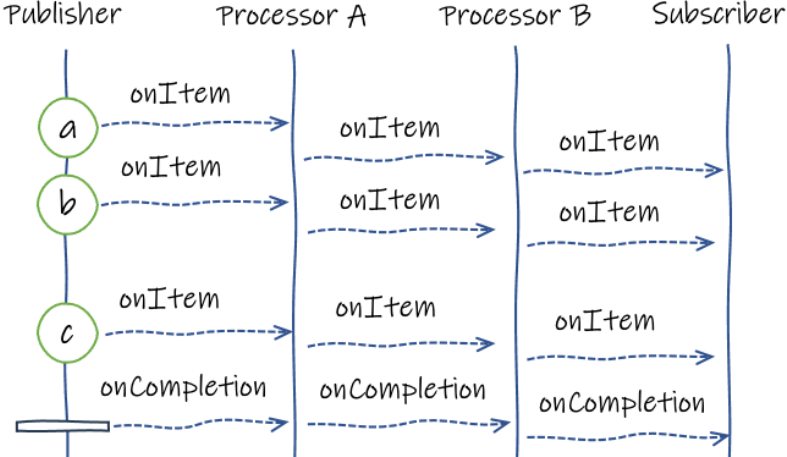
\includegraphics[width=0.9\textwidth]{EventFlow}
  \caption{Exemplarische Abbildung eines Event Flow in der Reactive Programming-Bibliothek Mutiny \parencite{MutinyEventFlow}}
  \label{fig:eventflow_mutiny}
\end{figure}

Reaktive Programmierung verinnerlicht das Konzept von nicht-blockierender bzw. asynchroner Ein- und Ausgabe.
Dabei wird, statt wie bei synchroner bzw. blockierender Ein- und Ausgabe die restliche Ausführung des Programms
zu blockieren bis die Datenübertragung abgeschlossen ist, nach dem Start der Übertragung bereits begonnen die Teile des
Programms auszuführen, die nicht von dem Ergebnis der I/O Operation abhängen.

\begin{lstlisting}[caption=Pseudocode Nonblocking I/O (NIO), captionpos=b, label=lst:NIO_Pseudocode]
NonBlockingDatabaseRequest().subscribe(print("req finished"))
NonBlockingDatabaseRequest2().subscribe(print("req 2 finished"))
print("hello world")
\end{lstlisting}
In Listing \ref{lst:NIO_Pseudocode} kann durchaus zuerst \verb|hello world| ausgegeben werden, da die gestarteten Datenbank-Anfragen die
restliche Programmausführung nicht blockieren. Wenn statt \verb|hello world| versucht würde, die Ergebnisse einer der Datenbank-Abfragen
darzustellen wäre das Ergebnis möglicherweise eine Exception oder \verb|null|, da die Anfragen zur Zeit der Ausführung von Zeile 3 noch nicht notwendigerweise
abgeschlossen sind. Das ist ein gängiger Fehler beim Arbeiten mit asynchronen, nicht-blockierendem Programmcode.

\subsection{Vorteile und Nachteile}
\label{subsec:vorteile_nachteile}

Die Vorteile der Nutzung von einigen wenigen \verb|kernel threads| als \verb|IO Threads| gegenüber eines ganzen Threadpools
an \verb|kernel threads|, um einen \verb|kernel thread| an jede HTTP-Anfrage zu binden, liegen insbesondere in den Antwortszeiten bei
hoher Last und dem Ressourcenverbrauch.
Umso weniger \verb|kernel threads| gleichzeitig aktiv sind, umso weniger Threadwechsel auf Betriebssystemebene
gibt es auch pro CPU-Kern, wodurch die Antwortzeiten von Anwendungen wesentlich besser mit der Erhöhung der Last skalieren können,
da Threadwechsel nicht mehr der limitierende Faktor sind und jeder \verb|IO Thread| wesentlich mehr CPU-Rechenzeit nutzen kann.
Darüber hinaus sinkt auch der allokierte Speicher deutlich
\footnote{Eine 64 Bit-JVM reserviert auf Linux-und Solaris-Systemen standardmäßig 1 MB Speicher für den Threadstack eines Threads}
und der Grad der Parallellität wird nicht mehr von der Anzahl der verfübaren Threads begrenzt.

Die Umstellung auf das reaktive Programmierparadigma erfordert allerdings eine Änderung in der Denk- und Herangehensweise bei der
Entwicklung von Softwarekomponenten. Denn reaktive Komponenten haben in der Regel keinen Zustand,
sondern reagieren lediglich auf interne Änderungen in den zugrundeliegenden Datenströmen.
Die bisherigen Programmabläufe müssten daher als reaktive Pipelines neu konstruiert werden.

Darüber hinaus ist reaktiver Code schwieriger zu debuggen und zu testen als imperativer Code, denn die Programmlogik die in den einzelnen Operatoren
der \verb|Pipes| einer \verb|Pipeline| aufgerufen wird, besteht in der Regel aus anynomen Funktionen und ist daher schwierig im Stack Trace einer
\verb|Pipeline| zurückzuverfolgen.
Während \verb|Event Flows| bei kleinen Pipelines noch zu überblicken sind, können komplexe Pipelines, die sich über die ganze Anwendung erstrecken,
schnell zu Wartbarkeits- und Verständnisproblemen führen.
Reaktive Programmierung ist zudem mit einer steilen Lernkurve verbunden. Dies liegt unter anderem an dem aktuellen Interesse an skalierenden
Anwendungen und der damit oftmals einhergehenden falschen Verwendung von Begriffen und der Überladung des Begriffs \verb|Reactive Programming|.
Aber auch die Funktionsweise von asynchronen Code (siehe Listing \ref{lst:NIO_Pseudocode}) kann zu schwer nachvollziehbaren und
reproduzierbaren Fehlern führen, wie beispielsweise das Auslösen einer NullPointer-Exception weil falsch strukturierter Code
auf Daten eines Services zugegreift die bei hoher Latenz zur Ausführungszeit noch nicht vorhanden sind, bei niedriger Latenz
allerdings schon.
Außerdem gibt es, Stand dieser Arbeit, kaum allgemeine, Herstellerunabhängige Fachliteratur zum Thema, wodurch sich viele verschiedenen Nomenklaturen und Vorgehensweisen der verschiedenen Anbieter von
Reaktive-Programming-Bibliotheken (siehe Kapitel \ref{subsec:java_ökosystem}), die sich größtenteils vor dem \verb|Reactive Streams|-Standard entwickelt haben, etabliert haben
und sich nicht klar voneinander abgrenzen.

Ein weiteres Problem besteht bei der Integration in bestehende Enterprise Anwendungen. Bibliotheken und Konzepte die Themen wie
Security, Transaktionen oder Tracing behandeln, führen oft immernoch blockierenden, threadgebundenen Code aus.
Jede Schicht einer Anwendung muss reaktiv konzipiert sein, da die Verarbeitung einer Anfrage, die blockierenden Code aus einer der
Schichten aufruft, ansonsten den ausführenden IO-Thread blockieren kann, wodurch dieser keine weiteren Anfragen bearbeiten kann und somit die gesamte Anwendung blockiert.
\newline\newline
Die wesentlichen Vor-und Nachteile lassen sich wie folgt zusammenfassen:
\newline
\newline
Vorteile
\begin{itemize}
  \item Die Antwortzeiten sind für hohe Lasten geringer, da deutlich weniger Threadwechsel gemacht werden müssen und jeder Thread
        mehr Rechenzeit bekommt
  \item Der Speicherverbrauch ist geringer, da weniger Threads genutzt werden
  \item Der Grad der Parallellität ist nicht von der Anzahl der Threads begrenzt
\end{itemize}
Nachteile
\begin{itemize}
  \item Asynchroner Code ist schwieriger zu schreiben, lesen, testen und zu debuggen als imperativer Code
  \item Sehr aufwendig in bestehende klassische Enterprise-Anwendungen zu integrieren
  \item Reaktive Anwendungen müssen in jeder Schicht reaktiv sein (Transaktionen, Security, Datenbanktreiber)
  \item Blockierende I/O-Operationen führen zur Blockierung des IO-Threads und damit zur Blockierung der gesamten Anwendung
\end{itemize}

\subsection{Reaktive Datenströme}
\label{section:reaktive_datenströme}
In einer typischen asynchronen Verarbeitungskette von, potenziell unbegrenzten, Datenströmen
bestehend aus einem Sender und Empfänger bzw. Publisher und Subscriber kann es vorkommen,
dass der Sender Daten schneller an den Empfänger verschickt, als dieser sie verarbeiten kann.
Zwei \verb|naive| Ansätze mit einer Überlastung des Empfängers umzugehen wären:
\begin{enumerate}
  \item Nur der Empfänger reagiert auf eine Überlast. Diese kann sich in einem Speicherüberlauf äußern oder, falls der Puffer des Empfängers eine Größenbeschränkung
        hat, im Verlust der empfangenen Daten
  \item Der Sender begrenzt im vornherein die Datenmenge, die er an den Empfänger schickt. Da der Sender allerdings in der Regel nicht weiß wieviel der Empfänger
        verarbeiten kann, sendet er entweder zuviel (es entsteht eine Überlast), oder er sendet zuwenig wodurch der Durchsatz geringer ist als nötig \parencite{JavaSpektrum2015}
\end{enumerate}
Die Lösung für dieses Problem wird \textit{Backpressure} genannt.
Dabei fordert der Empfänger die Daten entsprechend seiner Kapazitäten vom Sender an, wodurch dieser weiß wieviele Daten er maximal versenden darf.
Diese Mitteilung muss asynchron geschehen, da bei einer synchronen Kommunikation der Backpressure die Vorteile der asynchronen, reaktiven Datenverarbeitung
negiert würden.
Da große Anwendungen aus mehreren Schichten (bspw. Routing-Schicht, Persistenzschicht, Geschäftslogik) bestehen und somit zwischen
dem Sender und Empfänger mehrere Komponenten liegen können, muss jedes
Element der Verarbeitungskette nichtblockierendes, asynchrones Verhalten implementieren, da ansonsten der Rest der Kette blockiert würde.

Aus der Intention einen Standard für die asynchrone Verarbeitung von Datenströmen mit nicht-blockierender \textit{back pressure}
zu schaffen, ging die \textit{Reactive Streams}-Initiative hervor.
Innerhalb dieser Initiative haben sich mehrere Arbeitsgruppen gebildet, welche die grundlegenden Semantiken erarbeitet haben und
sie in Form einer eigenen Spezifikation namens \textit{Reactive Streams} für die JVM veröffentlicht haben.\parencite{ReactiveStreams}
Diese API wurde anschließend in Java 9, als Schnittstelle namens \textit{Flow-API} dem JDK hinzugefügt.
Die \textit{Flow-API} entspricht der \textit{Reactive Streams} Spezifikation und stellt (nur) Interfaces zur Verfügung mit denen eine
asynchrone, nicht blockierende Verarbeitung von (unbegrenzten) Datenströmen mit \textit{back pressure} auf der JVM implementiert werden kann.
\parencite{OracleFlow}.
\footnote{Nicht zu Verwechseln mit den Java-Streams durch die Collection-API ab Java 8. Diese sind zur Auswertungszeit in ihrer Größe begrenzt und
  nach der Abarbeitung liegt statt eines Streams eine Collection vor}

\subsubsection{Java Flow-API}
\label{subsection:java_flow_api}
Die Flow-API fügt die nicht instanziierbare,Klasse \verb|java.util.concurrent.Flow| zur Standardbibliothek hinzu. Sie enthält 4 Interfaces um das,
vom \textit{Reactive Streams}-Projekt standardisierte, beschriebene Publisher-Subscriber Model des Daten- bzw. Eventflusses
(siehe Listing \ref{lst:eventflow_pseudocode} und Abbildung \ref{fig:eventflow_mutiny}) mit \verb|backpressure|
von reaktiven Anwendungen auszudrücken:
\begin{enumerate}
  \item Publisher
  \item Subscriber
  \item Subscription
  \item Processor
\end{enumerate}

Die \verb|Flow|-Klasse erlaubt es Komponenten zu implementieren die Teil von reaktiven Pipelines sein können, in denen
\verb|Publisher| Elemente produzieren, die von einem oder mehr \verb|Subscriber| konsumiert werden. Die Beziehung zwischen einem
\verb|Publisher| und \verb|Subscriber| wird durch eine \verb|Subscription| abgebildet.
Während ein \verb|Publisher| theoretisch eine unbegrenzte Menge an Events liefern kann, wird er eingeschränkt durch den
\verb|Backpressure|-Mechanismus. Dadurch liefert der \verb|Publisher| immer nur soviele Elemente wie vom \verb|Subscriber| gefordert.
Der \verb|Publisher| erlaubt einem \verb|Subscriber| sich bei ihm zu registrieren um über die herausgegebenen Events informiert zu werden.
Die Kontrolle über den Fluss an Elementen (flow control), inklusive \verb|backpressure|, zwischen einem \verb|Publisher| und seinen \verb|Subscribern|
wird von der \verb|Subscription| verwaltet.
In Listing \ref{lst:java_flowapi} werden die 4 Interfaces der Flow-API dargestellt:
\begin{lstlisting}[language=java, caption=Die Klasse java.util.concurrent.Flow, captionpos=b, label=lst:java_flowapi]
@FunctionalInterface
public static interface Flow.Publisher<T> {
	public void subscribe( Flow.Subscriber<? super T> subscriber );
}
public static interface Flow.Subscriber<T> {
	public void onSubscribe( Flow.Subscription subscription );
	public void onNext( T item );
	public void onError( Throwable throwable );
	public void onComplete();
}
public static interface Flow.Subscription {
	public void request( long n );
	public void cancel();
}
public static interface Flow.Processor<T,R>
extends Flow.Subscriber<T>, Flow.Publisher<R> {
}
\end{lstlisting}\parencite[Kapitel 5.11]{JavaSE9StandardBibliothek}

Die vier \gls{callback}(*)-Methoden des \verb|Subscriber|-Interface werden vom \verb|Publisher| aufgerufen sobald eines der jeweiligen Events ausgelöst wird.
Die Events müssen dabei immer in der gleichen Reihenfolge veröffentlicht (und die jeweiligen Callback-Methoden ausgeführt) werden:
\begin{enumerate}
  \item onSubscribe
  \item onNext*
  \item (onError | onComplete)?
\end{enumerate}
Die Notation bedeutet, dass \verb|onSubscribe| immer als erstes aufgerufen werden muss, gefolgt von einer beliebigen Anzahl an
\verb|onNext|-Aufrufen. Dieser Eventstrom kann theoretisch ewig weitergehen, oder durch ein \verb|onComplete|-Aufruf beendet werden, welches
signalisiert das keine weiteren Elemente mehr vom \verb|Publisher| produziert werden.
Im Fehlerfall wird vom \verb|Publisher| das \verb|onError|-Callback aufgerufen.

Sobald sich ein \verb|Subscriber| bei einem \verb|Publisher| registriert, wird zuerst die \verb|onSubscribe|-Methode aufgerufen und dann ein
\verb|Subscription|-Objekt zurückgegeben. Ein \verb|Subscription|-Objekt wird nur von genau einem \verb|Subscriber| und einem \verb|Publisher| genutzt
und bildet die einzigartige Beziehung zwischen ihnen ab.

Der \verb|Subscriber| kann die erste Methode des \verb|Subscription|-Interfaces nutzen um den \verb|Publisher| zu informieren, dass er bereit
ist eine gegebene Anzahl an Events zu verarbeiten (backpressure). Mit der \verb|cancel|-Methode kann er die \verb|Subscription| abbrechen und dem \verb|Publisher|
somit mitteilen das er nicht länger Events erhalten will.
\parencite{JavaSEFlow}

Das \verb|Processor|-Interface erweitert \verb|Publisher| und \verb|Subscriber| ohne das weitere Methoden implementiert werden müssen.
Dieses Interface repräsentiert eine Transformation der Events, die durch den
reaktiven Datenstrom verarbeitet werden (siehe Listing \ref{lst:eventflow_pseudocode}).
Klassen die dieses Interface implementieren repräsentieren in der Regel die Operatoren einer Reactive Programming-Bibliothek.
Sobald ein \verb|Processor| ein Fehler erhält kann er sich entweder davon erholen oder direkt das onError-Signal an seinen
Downstream-Subscriber propagieren. Ein typischer Lebenszyklus eines reaktiven Datenstroms mit der Flow-API wird in
Abbildung \ref{fig:flow-api} gezeigt.
\begin{figure}[ht!]
  \centering
  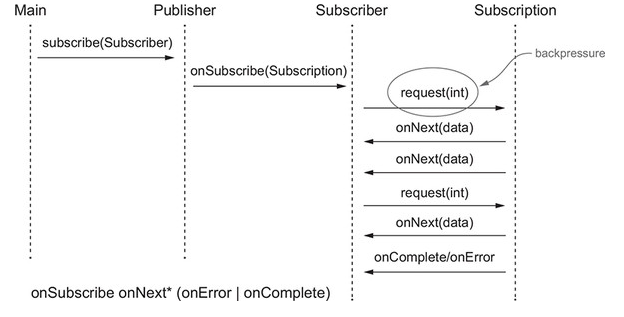
\includegraphics[width=0.9\textwidth]{flow-api_manning.PNG}
  \caption{Lebenszyklus eines reactive streams mit der Flow-API \parencite[Kapitel 17,  Figure 17.3]{JavaInAction}}
  \label{fig:flow-api}
\end{figure}
\newpage

\subsection{Reaktive Systeme}
\label{subsection:reaktive_systeme}
Anforderungen an große Softwaresysteme haben sich in den letzten Jahren stark verändert:
\begin{itemize}
  \item Antwortzeiten in Millisekunden statt im Sekundenbereich
  \item Datengrößen in Petabytes statt Gigabytes
  \item 100\% Verfügbarkeit statt stundenlange Wartungsarbeiten
  \item Deployment auf einer Vielzahl von Plattformen und cloud-basierten Clustern mit tausenden Multikernprozessoren
\end{itemize}

Unternehmen aus verschiedenen Bereichen haben sich voneinander unabhängig an diese Kriterien angepasst und Architekturmuster
erarbeitet, mit denen robuste, belastbare und flexible Softwaresysteme entwickelt werden können, die die modernen Anforderungen
erfüllen.

2014 wurde mit dem \verb|Reactive Manifesto| versucht diese Ansätze der Systemarchitektur in Form eines Manifests zusammenzuführen
und daraus allgemeingültige Systemattribute abzuleiten.

\subsubsection{Eigenschaften}
\label{subsubsec:reaktive_systeme_eigenschaften}
Laut des \verb|Reactive Manifesto| sind Systeme reaktiv wenn sie folgende Eigenschaften besitzen:
\begin{itemize}
  \item Reaktionsschnell
  \item Widerstandsfähig (gegen Fehler)
  \item Elastisch
  \item Nachrichtengesteuert
\end{itemize}
Solche Systeme sind, laut den Autoren, flexibler, stärker entkoppelt und würden besser skalieren als herkömmliche, nicht-reaktive Systeme.
Dies mache sie leichter zu entwickeln, zugänglicher für Veränderungen und deutlich fehlertoleranter.
\newline\newline
Die Autoren definieren die genannten Systemeigenschaften wie folgt:
\paragraph{Antwortbereit}Das System reagiert, falls überhaupt möglich, zeitgerecht. Antwortbereitschaft ist dabei die Grundlage für Funktion und
Benutzbarkeit. Es ermöglicht das schnelle Erkennen und Behandeln von Fehlern, indem verlässliche, zeitliche Obergrenzen für die Antworten von
Komponenten innerhalb des Systems geschaffen werden. Sobald eine Komponente nicht innerhalb des Zeitfensters antwortet, wird dies als Fehler gewertet und kann
entsprechend behandelt werden.
Der Fokus von reaktionsschnellen Systemen liegt auf konsistenten und schnellen Antwortszeiten. Darüber hinaus schaffen sie
verlässliche Obergrenzen um eine konsistente Qualität zu erreichen.
Dieses Verhalten simplifiziert Fehlerbehandlung, und erhöht das Vertrauen der Benutzer bezüglich Interaktion.

\paragraph{Widerstandsfähig/Fehlertolerant}Das System bleibt auch bei Fehlern reaktionsschnell. Das gilt nicht nur geschäftskritische, hochverfügbare Systeme -
jedes System das nicht Fehlertolerant ist, wird nach Fehlern nicht mehr reaktionsfähig sein.
Widerstandsfähigkeit wird durch Replikation von Funktionalität bzw. Redundanz, Eingrenzung von Fehlern, Isolation von Komponenten und
Delegation von Verantwortung realisierbar.
Fehler werden innerhalb einer Komponente eingegrenzt und die Komponenten sind voneinander isoliert. Dadurch bleibt das Gesamtsystem stabil, selbst
wenn eine einzelne Komponente versagt.
Die Wiederherstellung jeder Komponente (self-healing) wird an eine andere (möglicherweise externe) Komponente delegiert, und
Hochverfügbarkeit der Komponenten wird, wo notwendig, durch Redundanz gewährleistet.

\paragraph{Elastisch}Das System bleibt reaktionsschnell unter variierenden Arbeitslasten. Auf Änderungen der Arbeitslast wird durch
Anpassung der allokierten Ressourcen, insbesondere Replikation, reagiert. Das impliziert ein Systemdesign das keine zentralen Performance-Bottlenecks oder
Reibungspunkte hat, damit Komponenten problemlos repliziert und die Last darauf verteilt werden kann.
Reaktive Systeme unterstützen prädiktive, skalierende Algorithmen zur Ressourcenberechnung,
indem sie die Live-Messungen von Performance relevanten Systemmetriken als Eingabe nutzen.

\paragraph{Nachrichtenorientiert}Reaktive Systeme basieren auf dem asynchronen, nichtblockierendem Austausch von Nachrichten, um die Komponenten voneinander
abzugrenzen und dadurch eine loose Kopplung, Isolation und eine transparente Lokalisierung der Komponenten zu ermöglichen.
Aufgrund dieser Abgrenzung werden Fehler als Nachrichten an andere Komponenten delegiert.
Der Ansatz jegliche Kommunikation der Komponenten durch das Übermitteln von Nachrichten zu implementieren ermöglicht Elastizität,
indem er das Verteilen der Arbeitslast, die Kontrolle der Datenströme durch das Überwachen der Nachrichtenwarteschlangen zur Laufzeit
(\textit{message queues}) und, falls nötig, Anwenden von \textit{back pressure}, erlaubt.
Ortsunabhängigkeit bedeutet, dass Code und Semantik des Programms nicht davon abhängen, ob dessen Teile auf demselben Computer
oder verteilt über ein Netzwerk ausgeführt werden.
Reaktive nachrichtenorientierte Systeme erlauben eine effiziente Verwendung von Ressourcen, da Komponenten beim Ausbleiben von
Nachrichten vollständig inaktiv bleiben können, und sich nicht regelmäßig über neue Nachrichten informieren müssen.\parencite{ReactiveSystems}

Im Gegensatz zu Events haben Nachrichten immer ein klar definiertes Ziel.
Das bedeutet, dass sich ein ereignisgesteuertes System- oder Komponente auf adressierbare Event-Quellen konzentriert,
während ein nachrichtengesteuertes System auf adressierbaren Empfängern basiert.

In Abbildung \ref{fig:reactive-traits} wird das Zusammenspiel der Eigenschaften eines reaktiven Systems dargestellt.

\begin{figure}[ht!]
  \centering
  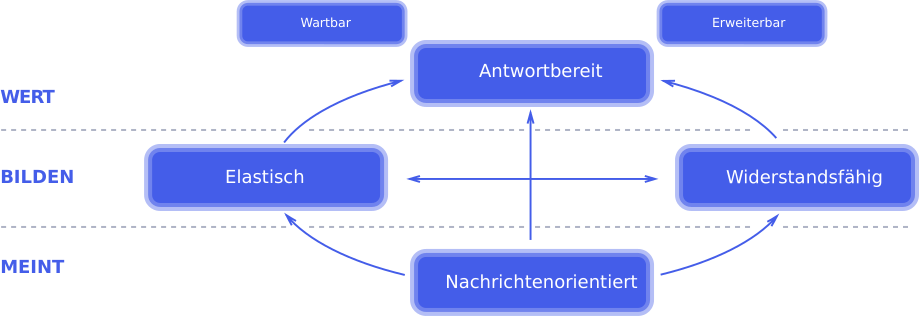
\includegraphics[width=0.9\textwidth]{reactive-traits-de}
  \caption{Zusammenspiel der Eigenschaften eines reaktiven Systems \parencite{ReactiveSystems}}
  \label{fig:reactive-traits}
\end{figure}
\newpage
\subsubsection{Abgrenzung zu reaktiver Programmierung}
\label{subsubsection:abgrenzung_reaktive_programmierung}
Aufgrund der steigenden Popularität von reaktiven Anwendungen ist der Begriff \verb|reaktiv| im Kontext der Softwareentwicklung
überladen und unterscheidet nicht zwischen \linebreak\verb|Reaktiver Programmierung| und \verb|Reaktiven Systemen|.

\verb|Reaktive Programmierung| ist eine ideale Technik zur Abbildung der internen Logik innerhalb einer Komponente, in Form von Transformationen
auf Datenströmen, um sowohl Performance, Ressourceneffizienz und Code-Verständlichkeit zu optimieren.

\verb|Reaktive Systeme| sind hingegen eine Menge von architektonischen Prinzipien, die die verteilte Kommunikation hervorheben und
Ansätze zur Realisierung von Fehlertoleranz und Elastizität liefern.

Ein gängiges Problem bei ausschließlicher Nutzung von \verb|Reaktiver Programmierung| besteht darin, dass die enge Kopplung
zwischen Verarbeitungsschritten (Transformationen) in einem eventgesteuerten Programm die geforderte Fehlertoleranz eines reaktiven Systems
schwer zu erreichen macht.
Die Transformationsketten bzw. \verb|Pipelines| sind kurzlebig und die Operatoren und Callback-Methoden innerhalb der \verb|Pipes|
sind anonym, also nicht adressierbar.

Das bedeutet, dass sowohl Erfolg, als auch Misserfolg bzw. Fehler direkt behandelt werden, ohne andere Komponenten darüber zu informieren.
Dieser Mangel an Adressierbarkeit erschwert die Wiederherstellung einzelner Phasen, da unklar ist, wo beziehungsweise ob Ausnahmen
propagiert werden sollten. Infolgedessen sind Fehler an kurzlebige Client-Anfragen und nicht an den
Gesamtzustand der Komponente gebunden – wenn eine der Phasen in der \verb|Pipeline| fehlschlägt, muss die gesamte \verb|Pipeline| neu
gestartet und der Client benachrichtigt werden. Dies steht im Gegensatz zu einem nachrichtengesteuerten reaktiven System, das
die Fähigkeit zur Wiederherstellung von Komponenten besitzt, ohne dass der Client benachrichtigt werden muss.

Ein weiterer Kontrast zum Ansatz eines reaktiven Systems ist, dass rein reaktive Programmierung zwar eine zeitliche Entkopplung,
aber keine räumliche Entkopplung ermöglicht. Zeitliche Entkopplung erlaubt gleichzeitige Verarbeitung, während räumliche Entkopplung
die Verteilung auf mehrere Systemkomponenten erlaubt. Dadurch können nicht nur statische, sondern auch dynamische Topologien
realisiert werden, was für die Elastizität eines reaktiven Systems essentiell ist.

Insgesamt ist \verb|reaktives Programmieren| eine sehr nützliche Technik, die in einer reaktiven Architektur genutzt werden kann.
Das Implementieren von Datenflüssen durch asynchrone und nichtblockierende Ausführung innerhalb eines Services bildet
die Basis eines reaktiven Systems, mehrere reaktive Services bilden aber noch kein reaktives System.

Sobald mehrere Services in einem reaktiven System miteinander arbeiten sollen, müssen unter anderem Funktionalitäten wie
Datenkonsistenz, Serviceübergreifende Kommunikation, Versionierung, Orchestrierung, Fehlermanagement und Trennung von Verantwortlichkeiten
berücksichtigt werden.

\subsection{Java Ökosystem}
\label{subsec:java_ökosystem}
Im Java Ökosystem gibt es eine Vielzahl an Libraries und Frameworks mit denen
\verb|Reaktive Programmierung| und \verb|Reaktive Systeme| umgesetzt werden können.
Um in Java einzelne, asynchrone Prozesse zu implementieren, wird vom JDK die Future-API zur Verfügung gestellt.\parencite{OracleFuture}
Für die Verarbeitung von asynchronen (unbegrenzten) Datenströmen gibt es die Interfaces der Flow-API (siehe Kapitel \ref{subsection:java_flow_api}).
\parencite{OracleFlow}

Im Folgenden wird ein Überblick über die Vielzahl an Bibliotheken und Frameworks gegeben.

\subsubsection{Reaktive Datenströme - Bibliotheken}
\label{subsubsec:reactive_streams}
Da die Flow-API lediglich Interfaces bereitstellt, gibt es mehrere Implementierungen von \verb|Reaktiven Datenströmen|.
Zu den populärsten Bibliotheken zählen:
\begin{itemize}
  \item RxJava
  \item Spring Webflux
  \item Mutiny
\end{itemize}
Jedes Projekt unterscheidet sich dabei in den verwendeten Klassen - und Operatoren um die \verb|reactive streams|-Spezifikation
beziehungsweise die \verb|Flow-API| des JDK, und damit auch \verb|back pressure| zu implementieren.
Trotzdem sind sie interoperabel und bieten in der Regel Converter-Klassen an.
\begin{itemize}
  \item RxJava\footnote{Implementiert die Flow-API erst seit Version 2} - Flowable, Observable \parencite{RxJava}
  \item Project Reactor - Flux, Mono \parencite{ProjectReactor}
  \item Mutiny - Multi, Uni \parencite{Mutiny}
\end{itemize}

\subsubsection{Reaktive Systeme - Toolkits}
\label{subsubsec:reaktive_systeme}
Für die Entwicklung von reaktiven Systemen bieten sich mehrere Toolkits an.
sie implementieren bereits Mechanismen wie Messaging, Event Loops,
nichtblockierende Netzwerkkomponenten und Dateizugriffe, sowie umfangreiche Funktionen für Webanwendungen.
Zu den populärsten gehören:
\begin{itemize}
  \item Eclipse Vert.x \parencite{Vert.x}
  \item Akka \parencite{Akka}
  \item Reactor-Netty \parencite{ProjectReactor}
\end{itemize}
Sowohl \verb|Eclipse Vert.x| als auch Reactor-Netty nutzen dabei \verb|Netty|
(siehe Kapitel \ref{subsubsec:reactor_pattern}) als Low-Level Framework für \verb|Nonblocking I/O|.
Da das in dieser Arbeit verwendete Anwendungsframework \verb|Quarkus| auf \verb|Eclipse Vert.x| basiert, wird Vert.x im Folgenden genauer beschrieben:

\paragraph{Eclipse Vert.x}
Vert.x ist ein Toolkit für das Entwickeln von reaktiven Anwendungen auf der JVM und wird unter dem Dach der herstellerneutralen Eclipse Foundation entwickelt.
Da es sich nicht um ein Framework handelt, gibt es keine vordefinierte Grundlage für Anwendungen und dadurch kann es auch in bestehende Projekte
integriert werden.
Der Kern des Toolkits \verb|vertx-core| stellt APIs für asynchrones Programmieren, \verb|Nonblocking I/O|, Streaming und Zugriff zu
Netzwerkprokollen wie TCP, UDP, DNS HTTP oder WebSockets.
\begin{figure}[ht!]
  \centering
  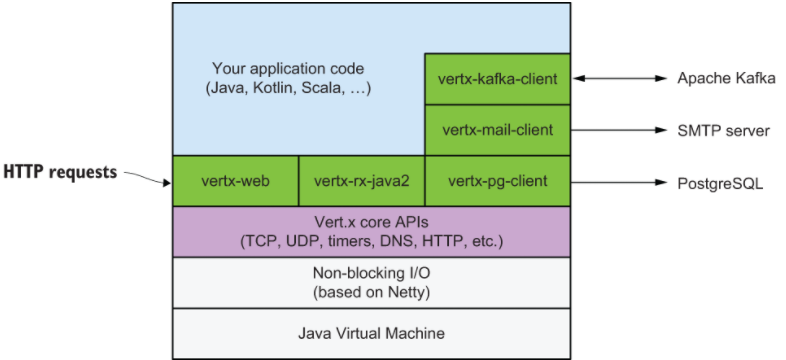
\includegraphics[width=1.0\textwidth]{vertx}
  \caption{Vert.x Struktur \parencite{Ponge2020}}
  \label{fig:vertx}
\end{figure}

Für die räumliche Entkopplung eines reaktiven Systems bietet Vert.x einen \verb|Event Bus|.
Der \verb|Event Bus| stellt ein verteiltes Peer-To-Peer Nachrichten System dar, welches sich über mehrere Serverknoten ersteckt.
Damit können verschiedene Komponenten eines Systems, unabhängig von der genutzten Programmiersprache, durch eindeutige Addressierung miteinander kommunizieren.
Auf jede Adresse können sich, ganz nach dem \verb|Publish-Subscribe|-Modell, mehrere Subscriber registrieren. Sobald Nachrichten an eine
Adresse veröffentlicht (published) werden, werden diese an jeden \verb|Subscriber| weitergeleitet.

Für die Resilienz eines reaktiven Systems verfügt Vert.x über einen Hochverfügbarkeits-Modus (high availablity, HA).
Dabei wird im Falle des Versagens einer Vert.x-Instanz die Anwendung auf eine andere Instanz innerhalb eines Clusters redeployed.
Darüber hinaus wird im Falle des Ausfalls einer Komponente durch einen \Gls{circuitBreaker}(*) vermieden, dass weitere Anfragen an diese
Komponente getätigt werden.\newline

Eine Implementierung des \verb|Reactor|-Pattern nutzt standardmäßig einen einzigen \newline\verb|Event loop thread|,
der in einer Schleife alle Events an die jeweils registrierten Event-Handler liefert.
Da durch einen einzigen \verb|Event loop thread| allerdings zu jeder Zeit auch nur ein CPU-Kern genutzt wird, kann
eine solche Implementierung Mehrkern-CPUs nur nutzen, indem mehrere Prozesse gestartet und verwaltet werden.

Statt einer einzigen Event Loop hält jede Vertx-Instanz, abhängig von der Anzahl der verfügbaren CPU-Kerne\footnote{1 Thread pro logischem CPU-Kern},
mehrere \verb|Event loop threads|. Diese Threads werden aus einem im vornherein erzeugten \verb|Event loop thread pool| entnommen.
\footnote{Die Größe des \textit{event loop thread pools} kann auch manuell überschrieben werden}

Um dieses Pattern vom Single Threaded Reactor-Pattern zu unterscheiden, wird es in der Vert.x-Dokumentation als \verb|Multi-Reactor Pattern| bezeichnet.
\parencite{Vert.xDocs}  \newline

Im Falle dass die Event Loop eines \verb|Event loop threads| durch \verb|Blocking I/O| blockiert würde, wird die Operation stattdessen auf einem
\verb|Worker thread|, aus einen im vornherein erzeugten \verb|Worker thread pool|, abgewickelt. Dieser Prozess bezeichnet \verb|Vert.x| als \verb|Dispatching|.
Durch \verb|Dispatching| entstehen natürlich Threadwechsel, aber es ermöglicht die Nutzung von Vert.x in bestehenden Projekten, die nicht komplett
auf \verb|Nonblocking I/O| basieren\parencite[Seite 2]{VertxArticle}.
Vert.x führt also zwei Thread Pools mit \verb|Kernel-Threads|, einen für \verb|Event loop threads|, dessen Größe der Anzahl der logischen CPUs entspricht,
und einen für \verb|Worker threads|, auf dem die Operationen abgearbeitet werden die die \verb|Event loop threads| blockieren würden.
\parencite{Vert.xOptions}

\subsubsection{Frameworks}
\label{subsubsec:frameworks}
Um komplette Web-Applikationen zu implementieren bietet sich der Gebrauch von Frameworks an, die Entwicklern viele grundlegende Architekturentscheidungen
abnehmen und bereits vorgefertigte Lösungen für Themen wie Authenfizierung, Routing, \Gls{ormg}(*), Security und Serialisierung anbieten oder
Lösungen von Drittanbietern integrieren und vorkonfigurieren.
Um reaktive Anwendungen und Systeme mit mehreren Services sinnvoll zu nutzen, ist es notwendig dass jede, für die Abarbeitung eines Requests relevante,
Anwendungsschicht und Komponente auch reaktiv ist und \verb|Nonblocking I/O| benutzt, sowie eine API bietet auf der
sich Event-Handler bzw. Subscriber registrieren können.

Die populärsten Frameworks mit einem komplett reaktiven Stack sind dabei:

\begin{itemize}
  \item Spring WebFlux
  \item Quarkus
\end{itemize}

Spring WebFlux nutzt dabei \verb|Project Reactor| und Quarkus \verb|Vert.x| als reaktive Engine. \parencite{QuarkusReactiveGettingStarted}
Da die exemplarischen Anwendungen dieser Arbeit (siehe Kapitel \ref{section:vergleich_reaktiv_blockierend}) das Quarkus-Framework nutzen, wird dies
im Folgenden genauer beschrieben:
\paragraph{Quarkus und native image}

Bei dem, in dieser Arbeit verwendeten, Framework \verb|Quarkus| handelt es sich laut Hersteller Red Hat, um ein
benutzerfreundliches, auf Entwickler abgestimmtes Java Framework, welches für Container-, Cloud- und Serverless-Umgebungen optimiert ist und nur wenig
Konfiguration benötigt, sowie nur die besten und hochwertigsten Java-Bibliotheken und Standards nutzt.
Dabei können die Anwendungen sowohl auf einer JVM (JVM mode) laufen, als auch, durch native Kompilierung mit vollständigem Stack,
als nativ ausführbare Anwendung: dem \textit{native image} (native mode).

Dafür nutzt Quarkus eine, von Oracle entwickelte, Technologie namens \verb|GraalVM|.
Dabei handelt es sich um eine polyglotte, virtuelle Maschine und Laufzeitumgebung die auf dem OpenJDK basiert, und über
JVMCI \footnote{Java Virtual Machine Compiler Interface} den C2-Compiler der zugrundeliegenden HotSpot-JVM durch den
polyglotten Graal Compiler ersetzt.\parencite{GraalVM}
Beim C2-Compiler handelt es sich dabei um einen aggressiv optimierenden \verb|just-in-time|-Compiler (JIT) für Serveranwendungen, bei denen es nicht auf
schnelle Startzeiten und geringen Ressourcenverbrauch, sondern auf höchsten Durchsatz ankommt.
Dabei wird der unoptimierte Bytecode während der Laufzeit in Maschinencode übersetzt und ausgeführt. Sobald eine Methode hinreichend oft
ausgeführt wurde, daher auch als \verb|JIT Warm up| bezeichnet, und der Profiler genügend Informationen gesammelt hat, kann der JIT-Compiler
sie entsprechend optimieren, bevor sie in Maschinencode übersetzt wird.
Der Graal Compiler kann als JIT-Compiler im JVM mode genutzt werden, als auch als \verb|ahead-of-time|-Compiler (AOT) im native mode.\newline

Um ein \verb|native image| zu erstellen wird mithilfe des GraalVM-Compilers vor der Kompilierung der Anwendung in Maschinencode, also \verb|ahead-of-time|,
ermittelt welche möglichen Pfade das Programm bei einem gegebenen Klassenpfad durchlaufen kann. Da dadurch nur die tatsächlich benötigten Klassen
kompiliert werden sind Programme, die mit \verb|native image| erstellt wurden, um einige Größenordnungen kleiner als die Summe aus
JDK und den benötigten Bibliotheken.
Allerdings dauert der Vorgang aufgrund der umfassenden Analyse auch wesentlich länger als die Übersetzung in Bytecode mit \verb|javac|.
Damit Entwickler sich bei Java Anwendungen auch weiterhin nicht um Speicher-und Threadverwaltung kümmern müssen, wird die \verb|SubstrateVM|, eine
leichtgewichtige virtuelle Maschine, in das \verb|native image| hineinkompiliert.
sie stellt Laufzeitkomponenten wie den Garbage Collector und den Thread Scheduler bereit.

Die Analyse vor dem Kompilieren erfolgt unter der \verb|closed world|-Annahme. Dabei wird angenommen das jeglicher Code der zur Laufzeit des Programms
erreichbar ist zur Build-Time des \verb|native image| bekannt sein muss. Dadurch verursachen jegliche Java-Features die erst zur Laufzeit,
und nicht bereits während des Builds,
auswertbar sind, wie beispielsweise Reflection oder statische Initialisierung mit Datumswerten, Probleme für die Ahead-of-Time-Übersetzung.

Um dem Compiler die notwendigen Informationen zur Unterstützung von Reflection mitzuteilen, können
diese über Konfigurationsdateien oder programmatisch über die GraalVM- und SubstrateVM-API hinterlegt werden.
Dadurch können auch Anwendungen und Libraries die starken Gebrauch von Reflection machen wie beispielsweise Hibernate, Netty oder Tomcat
so angepasst werden, dass sie in einem \verb|native image| genutzt werden können.
\parencite{GraalVMNativeImage}
Darüber hinaus verspricht Quarkus, mit seiner Container-first-Philosophie durch \textit{native images} bis zu 300 Mal schnellere Startzeiten
und nur ein Zehntel des Speicherbedarfs im Vergleich zu traditionellen Java-Frameworks wie Spring Boot, wodurch es eine signifikante Reduzierung
der benötigten Ressourcen und Kosten, im Gegensatz zu einer Java-Anwendung auf der JVM, im Cloud-Umfeld darstellt.
\parencite{RedHatQuarkusInfografik}

Allerdings ist der maximal, mögliche Durchsatz (noch) deutlich niedriger gegenüber Anwendungen im \verb|JVM-Mode|, da durch die AOT-Kompilierung
auf adaptive Laufzeitoptimierungen wie JIT-Compiling verzichtet wird.
Der Leiter des GraalVM-Projektes hat allerdings in einer Diskussion auf GitHub erwähnt, dass es durch Profile Guided Optimizations (PGO)
theoretisch durch durchaus möglich sei einen gleichwertigen Durchsatz und Laufzeitperformance zu erreichen\parencite{GraalWuerthinger}.

Bei PGO handelt es sich, wie bei JIT-Compiling auch, um Profiling-Daten die zur Laufzeit des Programms gesammelt werden.
Dafür wird ein erstes native image generiert und ausgeführt. Die hierbei ermittelten Profiling-Daten werden anschließend der
Generierung des zweiten native image als Parameter hinzugefügt\footnote{Im Gegensatz zu einer JVM-Anwendung liegt ein
  native image statt als Bytecode bereits als Maschinencode vor, und kann daher zur Laufzeit nicht optimiert werden}
wodurch die Optimierungen bereits während des Builds ausgeführt und in das executable hineinkompiliert werden.

Des Weiteren erlaubt Quarkus die Kombination von blockierendem und nicht blockierendem, reaktiven Code.
Dabei wird der Dispatching-Mechanismus von \verb|Vert.x| genutzt (siehe Kapitel \ref{subsubsec:reaktive_systeme}), sobald also eine
\verb|Blocking I/O|-Operation aufgerufen wird, wird diese auf einem \verb|Worker thread| abgewickelt, statt die \verb|Event Loop|, und damit den
gesamten \verb|Event loop thread| bzw. \verb|IO thread|, zu blockieren.
Für die reaktive Programmierung bietet Quarkus die bereits genannte Bibliothek \verb|Mutiny| an.\parencite{Quarkus}

\subsection{Alternativen}
\label{subsec:alternativen}
In Java 1.1 wurden Threads als sog. \verb|Green Threads| implementiert.
Dabei wurde die Möglichkeit Threads vom Betriebssystem, also \verb|Kernel threads|,
verwalten zu lassen gar nicht genutzt.
\verb|Green threads| waren stattdessen als \verb|user threads| implementiert,
dabei ist die Funktionalität
nicht im Kernel implementiert, sondern in einer Programmbibliothek im Userspace (siehe Kapitel \ref{subsubsec:user-threads}).
Da sich das Betriebssystem nicht um das Scheduling von user threads kümmert, wurde dies über einen eigenen
Scheduling-Algorithmus der JVM geregelt.\parencite{Oracle2010}
Ein \verb|Green Thread| existiert lediglich als Objekt innerhalb der JVM, und durch die virtuelle Speicherverwaltung entfallen
somit die aufwändigen, kostenintensiven Betriebssystemaufrufe beim
Erstellen eines Threads, sowie bei Threadwechseln.
Die Threadwechsel der \verb|Green Threads| erfolgten ausschließlich innerhalb des Main-Threads, weswegen keine echte Parallelität
realisiert werden konnte, da immer nur ein Prozessorkern genutzt wurde.
Während der Vorteil dieses Modells darin lag, dass es keine 'echten' parallelen Zugriffe auf eine Resource innerhalb des JVM-Prozesses geben konnte
und die Synchronisation von Datenzugriffen daher leicht war, überwog schließlich der Umstand, dass keine Nutzung von mehreren Prozessorkernen
durch Multithreading möglich war, weswegen \verb|Green Threads| ab Java 1.3 zugunsten von Kernel-Threads entfernt wurden.

Mit dem OpenJDK Projekt \verb|Project Loom| ist die Idee
wieder aufgegriffen worden, allerdings nun als Ergänzung zu Kernel-Threads.
Statt alle virtuellen Threads auf dem nativen Main-Thread auszuführen, werden diese von einer geringen Anzahl an
nativen \verb|worker threads|, die als Carrier\footnote{Quasi die Träger der virtuellen Threads} eingesetzt werden, ausgeführt.
Deren Anzahl ist so gewählt, dass alle CPU Kerne durch Multithreading dauerhaft benutzt werden können
\footnote{In der Praxis laufen natürlich noch andere Prozesse auf dem Server, deren Threads auch ausgeführt werden müssen.}
, aber so wenig Kontextwechsel wie möglich ausgeführt werden müssen.\parencite{Oracle2021}
\footnote{Im Idealfall würde auf jedem CPU Kern ein \textit{worker thread} laufen, ohne Threadwechsel}
Während ein nativer Thread in einer 64 Bit JVM auf Linux-Systemen standardmäßig 1 MB für den Threadstack reserviert
und zusätzlich noch Metadaten abspeichert, ist ein virtueller Thread
lediglich ein Objekt im virtuellen Speicher der JVM und benötigt sehr wenig Resourcen.
Aus diesem Grund können, bei entsprechend allokierten Heap-Speicher der JVM, durchaus mehrere Millionen virtueller Threads erzeugt werden, wohingegen
die bereits die Erstellung von 10.000 nativen Threads entweder den allokierten Speicher oder die Threadgrenze
des Betriebssystems überschreitet.

In Kapitel \ref{subsubsec:user-threads} wurde bereits die Problematik erwähnt, dass ein Kernel-Thread auch blockiert und somit
das Scheduling der Laufzeitumgebung nicht ausführen kann, wenn einer seiner virtuellen Threads eine blockierende I/O-Operation ausführt.
Dies würde bei mehreren Kernel-Threads bzw. Carrier wieder zu Threadwechseln seitens des Kernel-Schedulers führen.

Die vorgeschlagene Lösung besteht in der Nutzung einer asynchronen, nicht-blockierenden API für I/O Operationen seitens
der Anwendung bzw. der Laufzeitumgebung. Dadurch erhält der Aufrufer unverzüglich nach dem Start einer blockierenden I/O-Operation
innerhalb eines virtuellen Threads die Kontrolle zurück und kann währenddessen einen neuen virtuellen Thread bearbeiten.

\verb|Project Loom|s Ziel und großes Versprechen ist allerdings eine Lösung ohne die Nutzung von asynchronen APIs für I/O-Operationen
zu finden, da diese gerade bei großen Systemen schwierig zu warten und zu verstehen sind.

//continuations
//welche parts des jdks betroffen
//
https://entwickler.de/java/blick-in-die-fernere-zukunft



//TODO Virtueller Thread gibt die Kontrolle freiwillig über Continuation ab, ansonsten gäbe es ja hier dasselbe Problem
//wie bereits in \ref{subsubsec:user-threads} geschildert -> der main thread würde durch den user thread blockiert >
//kernel threadwechsel müsste erfolgen

Sobald ein virtueller Thread nun eine blockierende I/O Operation ausführt führt die Laufzeitumgebung automatisch einen
virtuellen Threadwechsel (siehe Kapitel \ref{subsubsec:threadwechsel}) durch und ermöglicht dem nativen Thread währendessen einen
anderen virtuellen Thread auszuführen.

Das große Versprechen des Projektes ist außerdem, das Entwickler keine asynchronen Programmierparadigmen (wie u.a. \textit{Reactive Programming})
nutzen müssen um die beschriebenen virtuellen Threads und die damit einhergehenden wesentlichen Performanceverbesserungen nutzen zu können.
Um dieses Versprechen zu halten werden virtuelle Threads, statt als Bibliothek eines Drittanbieters, in Form einer eigenen JDK Version bereitgestellt.
In dieser Version wurden viele Teile der Standardbibliothek die mit I/O-Operationen arbeiten so angepasst, dass virtuelle Threads statt Kernel-Threads
genutzt werden. Auf diese Weise können I/O-Operationen, wie beispielsweise der Aufruf einer Netzwerkfunktionalität, ohne Änderungen am Programm,
die virtuellen Threads nutzen und blockieren den darunterliegenden nativen Thread nicht mehr.

Jüngere Programmiersprachen wie Kotlin und Golang benutzen bereits virtuelle statt nativer Threads
für ihre Threading-Abstraktion \verb|coroutines|. \parencite{KotlinCoroutines, GoCoroutines}
\section {Vergleich reaktive \& imperative Anwendung}
\label{section:vergleich_reaktiv_imperativ}
Um zu prüfen, ob Leistungsfähigkeit und Skalierbarkeit einer reaktiven, auf dem \newline
\verb|Multi-Reactor-Modell| und \verb|Nonblocking I/O| basierenden,
Anwendung tatsächlich die einer traditionellen, auf dem \verb|Thread-per-Request Modell| und \verb|Blocking I/O| basierenden, Anwendung übertrifft, werden in
diesem Kapitel beide Ansätze hinsichtlich verschiedener Metriken in einem festen Zeitintervall miteinander verglichen.

Dafür werden sowohl die reaktive, als auch die nicht-reaktive Anwendung, in 5 Testreihen, jeweils zwei Lasttests unterzogen:
\begin{enumerate}
    \item Abfrage von statischen Daten
    \item Abfrage von dynamischen Daten (mit Datenbankanbindung)
\end{enumerate}
Dabei wird pro Lasttest eine Reihe an Lasten bzw. \textit{workloads} von einem Client-Host generiert und über eine feste Dauer in kleinen Zeitinvervallen
an einen ausgewählten HTTP-Endpunkt der Anwendung gesendet.
In dieser Zeit wird das Zeitinvervall vom Starten der Anwendung bis zur Beantwortung der ersten Anfrage,
der benötigte Arbeitsspeicher und CPU-Auslastung des Prozesses, der Durchsatz, sowie die Latenz gemessen.

Für Container- und Cloud-Umgebungen eignen sich, primär aus Kostengründen, Anwendungen die, statt auf hohen Durchsatz und lange Laufzeiten, auf
schnelle Startzeiten und geringen Ressourcenverbrauch setzen.
Aus diesem Grund werden die beiden Anwendungen sowohl im \textit{JVM mode} als auch im \textit{native mode}
(siehe Absatz \verb|Quarkus und native image| in Kapitel \ref{subsubsec:frameworks})
den beiden Lasttests unterzogen. Ingesamt ergeben sich also 4 Testszenarien pro Anwendung.

\subsection{Implementierung \& Systemaufbau}
\label{section:implementierung}
Die beiden Anwendungen implementieren mit dem Quarkus-Framework jeweils eine simple REST-Schnittstelle mit HTTP-CRUD Methoden
und einer angebundenen PostgreSQL-Datenbank.
Dabei ist vorallem die HTTP-Schicht von Interesse. Die HTTP-Unterstützung von Quarkus basiert auf einem reaktiven, nicht-blockierenden
Unterbau: der Vert.x Engine (siehe Kapitel \ref{subsubsec:reaktive_systeme}).
Jede HTTP-Anfrage wird auf einem der \textit{event-loop threads} bzw. \textit{IO threads}
verarbeitet und durch eine Routing-Schicht an den Anwendungscode weitergeleitet.
Je nachdem welcher Ansatz zur Implementierung des jeweiligen HTTP-Endpunktes gewählt wurde,
wird der abzuarbeitende Code dann auf einem blockierenden \textit{worker thread}, ganz nach dem \verb|Thread-Per-Request Modell|, aus dem
\textit{worker thread pool} (Servlet, \Gls{jaxrsg}(*)) oder, nach dem \verb|Multi-Reactor-Modell|, weiter auf einem der
\textit{IO threads} (Reactive Routes, Reactive Resteasy) ausgeführt.

\newpage
\begin{figure}[h]
    \centering
    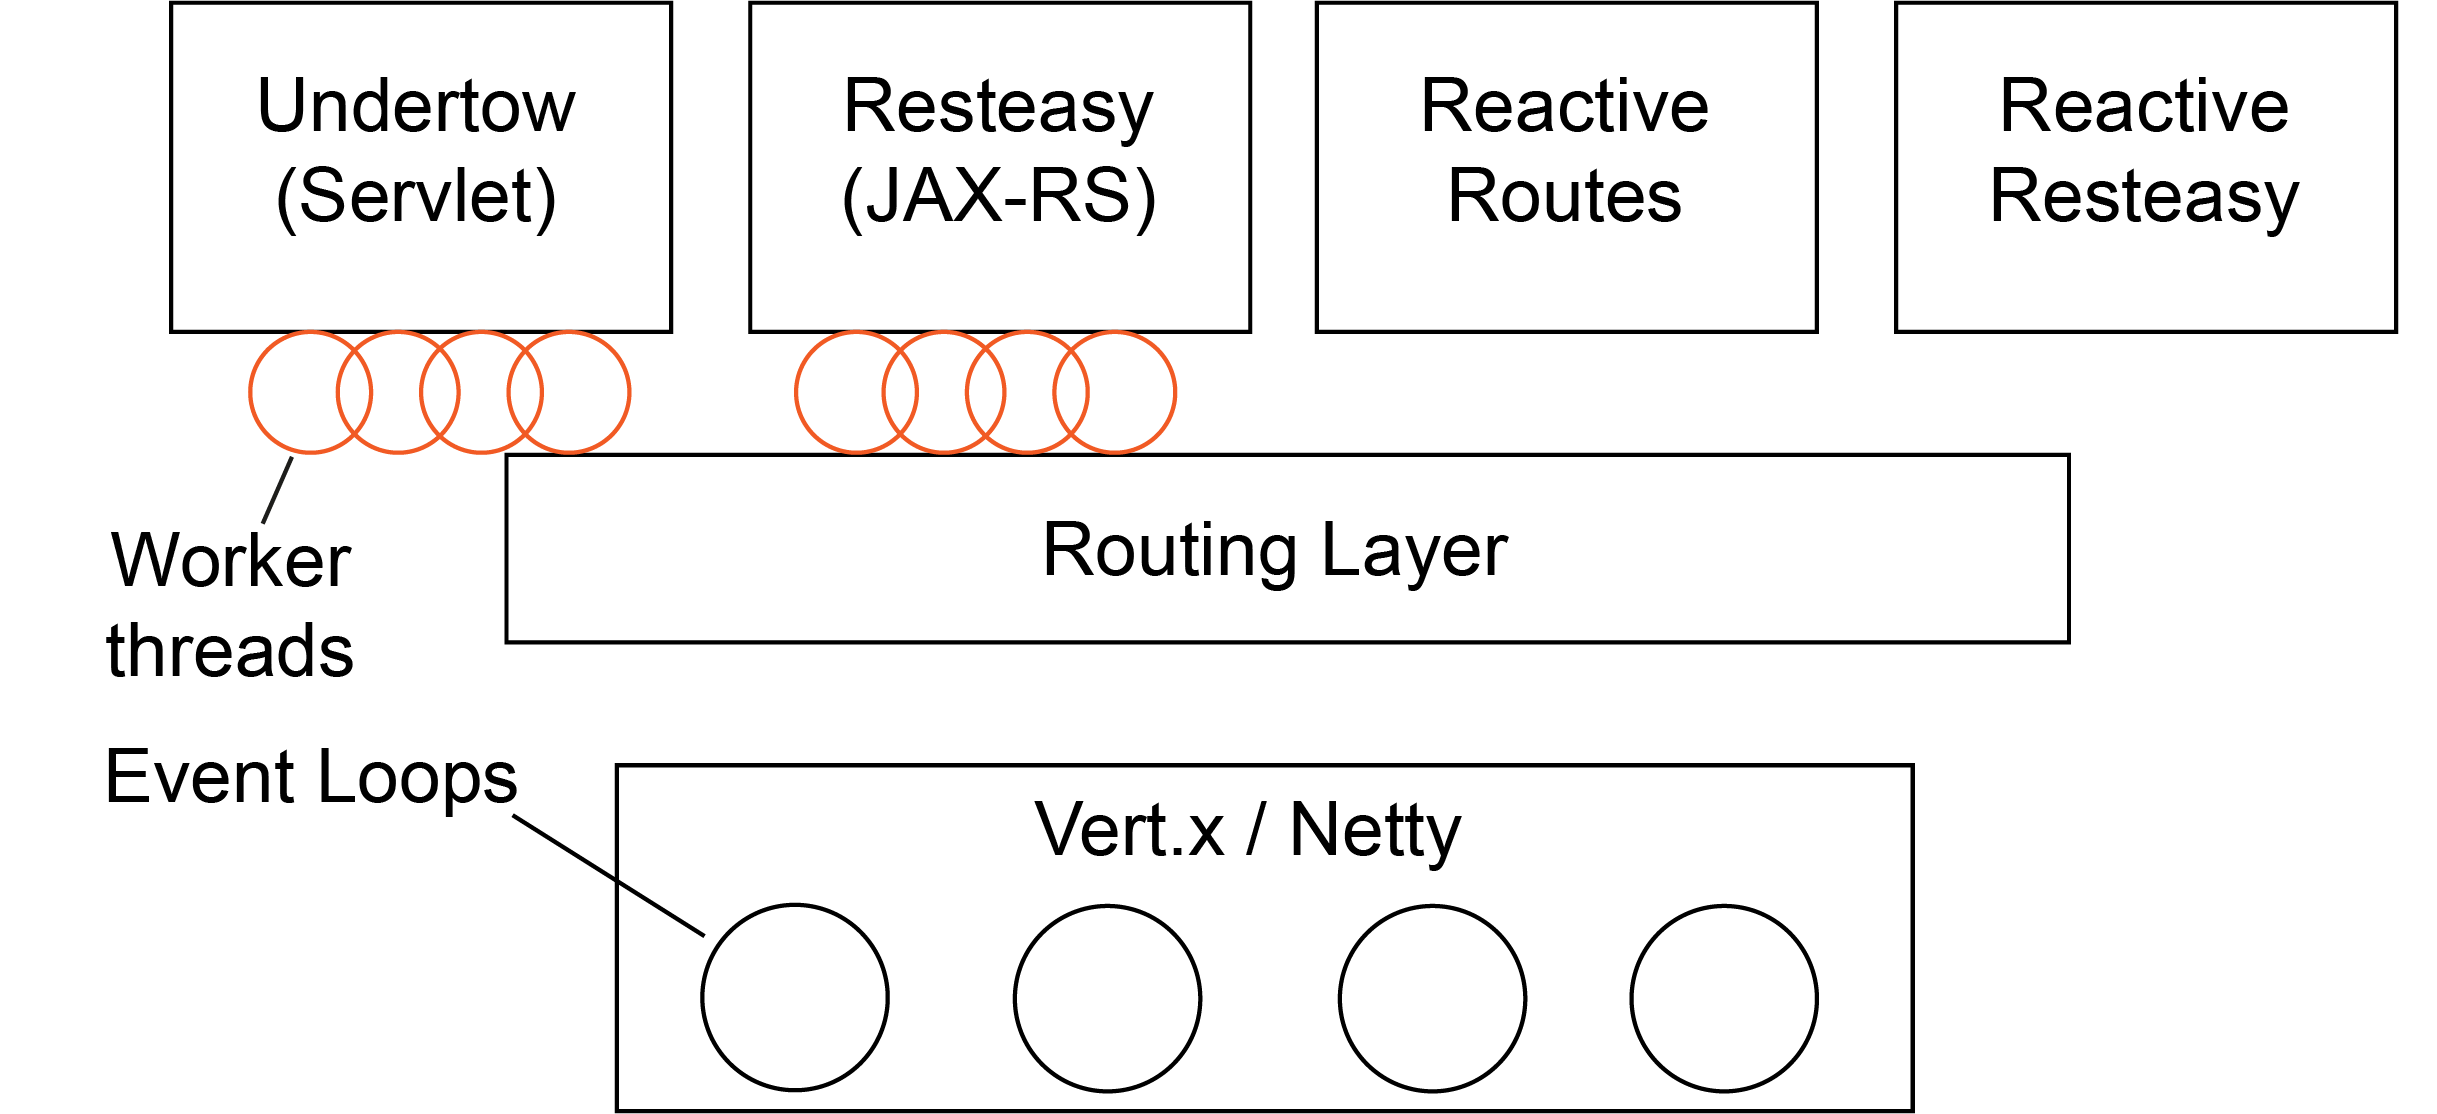
\includegraphics[width=0.9\textwidth]{Quarkus_HTTP_Layer}
    \caption{Quarkus HTTP-Schicht \parencite{QuarkusReactiveRoutes}}
    \label{fig:quarkus_http_schicht}
\end{figure}

Die \textit{IO threads} sind dafür zuständig alle IO-Operationen asynchron auszuführen und die jeweiligen EventListener bzw. Subscriber
auszulösen sobald die Operationen abgeschlossen sind.
Damit sich beide Anwendungen nahe an einer realen Java-EE CRUD REST-API orientieren, haben
sie (zusätzlich zu den grundlegenden Abhängigkeiten des Quarkus-Frameworks) folgende Projekt-Abhängigkeiten:
\begin{itemize}
    \item JAX-RS Implementierung
    \item \Gls{jsong}(*) Unterstützung
    \item PostgreSQL - Datenbanktreiber
    \item \Gls{jpag}(*) Implementierung
\end{itemize}

Diese Abhängigkeiten wurden vom Quarkus Maven-Repository sowohl in blockierender,
als auch in nicht-blockierender, reaktiver und in \verb|native image|-kompatibler Form bereitgestellt: \parencite{MavenQuarkusIO}
% space between the text and the left/right border of its containing cell is set to 18 pt
\setlength{\tabcolsep}{18pt}
% the height of each row is set to 1.5 relative to its default height
\renewcommand{\arraystretch}{1.5}
\begin{table}[ht!]
    \centering
    \begin{tabular}{| c | c | c |}
        \hline
                         & Blockierend      & Nicht-blockierend (reaktiv) \\
        \hline
        JAX-RS           & Resteasy         & Resteasy Reactive           \\
        \hline
        JSON             & Resteasy-Jackson & Resteasy-Reactive-Jackson   \\
        \hline
        Datenbanktreiber & JDBC-Postgresql  & Reactive-Pg-Client          \\
        \hline
        JPA-/ORM         & Hibernate-ORM    & Hibernate-Reactive          \\
        \hline
    \end{tabular}
    \caption{Tabelle mit den Abhängigkeiten beider Applikationen}
    \label{table:dependencies}
\end{table}

In Listing \ref{lst:update_reactive} und \ref{lst:update_blocking} ist jeweils die Update Methode der REST-APIs abgebildet, um den
Unterschied der beiden Paradigmen auf Code-Ebene darzustellen.

Dabei wird versucht eine Entity mit der übergebenen \verb|id| des API-Endpunktes
aus der Datenbank abzurufen und, falls eine Entity mit der \verb|id| gefunden werden konnte, dessen Name mit dem Wert
aus dem Request-Body der Anfrage zu überschreiben. Anschließend wird die Entity mit dem neuen Namen wieder in die Datenbank zurückgeschrieben
und HTTP-Statuscode 422 an den Client zurückgegeben. Falls keine Entity gefunden werden konnte, wird stattdessen
HTTP-Statuscode 404 zurückgegeben.

In der reaktiven Anwendung ist die gesamte Logik, sowie Fehler- und Nullprüfung in einer einzigen Pipeline abgebildet.
Da in diesem Beispiel Mutiny genutzt wird, wird der Rückgabetyp immer als \verb|Uni| oder \verb|Multi|-Objekt eines spezifischen Typs
angegeben. \verb|Uni| repräsentiert dabei einen Datenstrom der entweder ein Element oder ein Fehler-Event emittiert.
\verb|Multi| repräsentiert einen Datenstrom der entweder 0, 1, \verb|n| oder unendlich viele Elemente emittieren kann.
Der \verb|Subscriber| ist in diesem Fall der Aufrufer der \verb|update|-Methode und sorgt dafür, dass die Pipeline überhaupt ausgeführt wird.

Jede \verb|Pipe| bzw. \verb|Processor| der Pipeline der \verb|update|-Methode gibt ein \verb|Uni|, dieses kann entweder
vom Typ \verb|Void| (für null-Werte) oder von der jeweiligen Entität sein, an den Downstream weiter
\footnote{invoke() und call() sind Abkürzungen, um die Lesbarkeit zu verbessern\parencite{MutinyShortcuts}}.

\begin{lstlisting}[caption=Update Methode der reaktiven Anwendung, language=Java, captionpos=b, label=lst:update_reactive]
@PUT
@Path("{id}")
public Uni<Response> update(Long id, Fruit fruit) {
	if (fruit == null || fruit.getName() == null) {
		return Uni.createFrom().item(Response.status(422).build());
	}
	return fruitRepository.findById(id).onItem()
	.ifNotNull().invoke(storedFruit -> storedFruit.setName(fruit.getName())
	).call(storedFruit -> fruitRepository.update(storedFruit))
			.onItem().ifNotNull().transform(storedFruit ->
			Response.ok(storedFruit).build())
			.onItem().ifNull().continueWith(Response.status(Status.NOT_FOUND).build());
}
\end{lstlisting}
\begin{lstlisting}[caption=Update Methode der nicht-reaktiven Anwendung, language=Java, captionpos=b, label=lst:update_blocking]
@PUT
@Path("/{id}")
public Response update(Fruit fruit, @PathParam("id") Long id) {
	if (fruit == null || fruit.getName() == null) {
		return Response.status(422).build();
	}
	Fruit storedFruit = fruitRepository.findById(id);
	if (storedFruit == null) {
		return Response.status(Response.Status.NOT_FOUND).build();
	}
	storedFruit.setName(fruit.getName());
	fruitRepository.update(storedFruit);
	return Response.status(Response.Status.OK).build();
}
\end{lstlisting}

Der Projekt-Code dieser Arbeit kann von GitHub unter \url{https://github.com/ErikSimonsen/quarkus-iothread-workerpool} eingesehen und abgerufen werden.

\subsection{Testumgebung}
\label{section:testumgebung}
Für die Testumgebung werden zwei Systeme benötigt: der Client-Host und der Server-Host.
Dabei muss es sich um UNIX-Systeme handeln, da einige der verwendeten Werkzeuge nur auf diesen Systemen verfügbar sind.
Zudem müssen beide Systeme per SSH von einem (idealerweise vorhandenem) dritten System, dem User-Host
\footnote{Dies kann allerdings auch der Client-Host selber sein}
erreichbar sein, damit dieses den Testablauf in der korrekten Abfolge ausführen kann.
Der Einfachheit halber empfiehlt es sich, dass sich alle Geräte im gleichen Netzwerk befinden.
Beide Anwendungen verwenden Version 1.12.1 des Quarkus Frameworks, welches wiederrum Version 20.1 der GraalVM nutzt.
Um eine reproduzierbare Anwendungsumgebung und Ressourcenallokation zu ermöglichen, laufen beide Anwendungen auf dem Server-Host in
jeweils einem Docker-Container mit fest definierten Ressourcen:
\begin{itemize}
    \item Nutzung von 4 CPU-Kernen
    \item 1024 MB RAM
    \item 256 MB Heap Größe für den Java-Prozess
          \footnote{Seit Java 10 wird automatisch ~1/4 des Speicher Limits des Containers genutzt \parencite{Java10ReleaseNotes}}
\end{itemize}
Der jeweilige Docker-Container für die Postgresql-Datenbank allokiert:
\begin{itemize}
    \item 4 CPU-Kerne
    \item 2048 MB RAM
\end{itemize}

Die Größe des von Vert.x verwendeten \verb|Worker Thread Pools| (siehe Abbildung \ref{fig:quarkus_http_schicht}) beträgt standardmäßig 20 und bleibt
unverändert, die Größe des \verb|Event-Loop Thread Pools| hingegen wird für die Tests manuell auf 8 gesetzt, da die Anwendung durch die Ressourcenallokation
des Docker-Containers nur 4 CPU-Kerne nutzen darf und jeder dieser CPU-Kerne Hyperthreading unterstützt. \footnote{Wodurch jeder physische CPU-Kern über
    zwei logische CPUs verfügt} Damit kann die optimale Verteilung von einem \verb|Event-Loop Thread| bzw. \verb|IO-Thread| pro
logischer CPU erreicht werden.
Standardmäßig wird die Ressourcenbegrenzung durch Container von Vert.x nicht beachtet und die Anzahl der \verb|Event loop|-Threads auf die doppelte
Anzahl der verfügbaren CPU-Kerne des Container-Hosts gesetzt, weswegen es für ressourcenbegrenzte Container der beschriebenen Korrektur bedarf.
Der \verb|Worker Thread Pool| wird vom \verb|Thread-per-Request Modell| bzw. \verb|Blocking I/O| genutzt, während der \verb|Event-Loop Thread Pool| von der
reaktiven Anwendung bzw. \verb|Nonblocking I/O| genutzt wird.

Die Anwendung, die auf dem Client-Host die \textit{work load} für die beiden zu testenden Anwendungen generiert,
nutzt in dieser Testumgebung 4 Threads.
\footnote{Welche Laufzeitumgebungen und Tools für die Tests auf den jeweiligen Hosts vorhanden sein müssen, und wie diese installiert werden
    wird in der README.md-Datei des Projektverzeichnisses beschrieben.}

Da die Messergebnisse je nach verwendeter Hardware der Client- und Server-Hosts durchaus variieren können werden im Folgenden
die Systemspezifikationen der verwendeten Systeme des Authors gelistet:
\begin{table}[ht!]
    \centering
    \begin{tabular}{| c | c |}
        \hline
        Server-Host                                                  \\
        \hline
        CPU's          & AMD Ryzen 7 2700x eight-core processor x 16 \\
        \hline
        RAM            & 16GB                                        \\
        \hline
        Speicher       & 1,5 TB                                      \\
        \hline
        Betriebssystem & Fedora 34 (Workstation Edition)             \\
        \hline
        Kernel         & Linux version \verb|5.12.14-300.fc34.x86_64|   \\
        \hline
    \end{tabular}
    \caption{Systemspezifikationen der verwendeten Server-Maschine}
    \label{table:system_host}
\end{table}

\begin{table}[ht!]
    \centering
    \begin{tabular}{| c | c |}
        \hline
        Client-Host                                                \\
        Hardware       & Acer Aspire VN7-591G                      \\
        \hline
        CPU            & Intel® Core™ i5-4210H CPU @ 2.90GHz × 4   \\
        \hline
        RAM            & 8GB                                       \\
        \hline
        Speicher       & 500 GB                                    \\
        \hline
        Betriebssystem & Fedora 34 (Workstation Edition)           \\
        \hline
        Kernel         & Linux version \verb|5.12.14-300.fc34.x86_64| \\
        \hline
    \end{tabular}
    \caption{Systemspezifikationen der verwendeten Client-Maschine}
    \label{table:system_client}
\end{table}

\subsection{Testvorgehen / Testaufbau}
\label{section:vorgehen}
Der im Folgenden erläuterte Versuchsaufbau basiert auf einer, vom Autor erweiterten, Architektur die vom Quarkus-Entwicklerteam
zur Erstellung von verschiedenen Benchmarks für den Quarkus Technologie-Stack genutzt wurde.
\parencite{QuarkusBlog, QuarkusJohnaohara}

Um den gesamten Versuchsablauf zu automatisieren und über mehrere Server zu steuern wird ein Tool namens qDup eingesetzt.
Damit können Shell-Kommandos als Skripte gruppiert, und verschiedenen Hosts je nach Rolle zugewiesen werden.
\footnote{Die qDup Skripte mit dem gesamten Testablauf können im Verzeichnis \textit{/scripts/qDup} des Quellcodeverzeichnisses eingesehen und
    angepasst werden.}
Um dem Ablauf korrekt zu steuern werden Signale definiert die ein Host sendet, und auf die die anderen Hosts warten um ihrerseits
weitere Skripte auszuführen.
\footnote{Beispielsweise sollte der Server-Host erst anfangen den Java-Prozess zu überwachen, sobald der Client-Host die \textit{workload}
    generiert und nicht bereits davor}

Wie bereits in \ref{section:testumgebung} angedeutet, nutzt qDup SSH um auf die jeweilige Hosts zuzugreifen.

Im ersten Schritt \textit{build applications} wird auf dem Server-Host das Quellcodeverzeichnis geklont und beide Anwendungen werden, für
ein einfaches Deployment in den Docker-Container, jeweils als \gls{uber-jar}(*) und \verb|native image| gebaut.

Anschließend wird über ein JavaScript-Skript, welches in der Laufzeitumgebung Node.js läuft,
die \verb|Mean Start Time to First Request|, also das durchschnittliche Zeitintervall zwischem dem Start einer Anwendung bis
zur Verarbeitung der ersten Anfrage, mehrfach gemessen und als Textdatei gespeichert.
Dabei wird die gebaute Anwendung, ohne Docker-Container, auf dem Server-Host gestartet und die Zeit genommen. Anschließend werden in einer Schleife
solange Anfragen an einen Endpunkt der Anwendung gestellt bis das Ergebnis ein Statuscode 200 ist, was den Endpunkt der Messung markiert.
Aus den gemessenen Startzeiten wird in der Auswertung der Daten anschließend der Durchschnitt gebildet, um somit die \verb|Mean Start Time to First Request|
der Anwendung zu erhalten.

Darüber hinaus werden die Docker-Container der Datenbank
\footnote{Nur beim Test mit dynamischen Daten} und der beiden REST-APIs gebaut.

Beim zweiten Schritt \textit{run applications} wird der Docker-Container der jeweiligen Anwendung gestartet und anschließend signalisiert,
dass die Anwendung nun bereit ist.
Daraufhin wird auf dem Client-Host das Skript \textit{generate load} gestartet.
Die \textit{workload} ist hier definiert als die Anzahl der, an den Server-Host, versendeten \textit{HTTP-Anfragen pro Sekunde}.
Für das Generieren und Übermitteln der \textit{workload} wird das Werkzeug \textit{wrk2} genutzt, welches das
bewährte HTTP-Benchmarking Tool \textit{wrk} um folgende Funktionen erweitert:
\begin{enumerate}
    \item Konstanter \textit{workload} Durchsatz
    \item Korrekteres Messverfahren der Antwort-Latenz durch Vermeidung von \verb|Coordinated Omission|
    \item Hochexaktes Messen durch \Glsuseri{hdrHistogramm}(*)
\end{enumerate}\parencite{Wrk2, Wrk}

\paragraph{Coordinated Omission Problem}
Der Begriff \verb|Coordinated Omission Problem| wurde von Gil Tene, CTO und Mitgründer von Azul Systems, um 2012 geprägt.
Koordinierte Auslassung beschreibt in diesem Kontext das Problem, wenn ein Messsystem sich mit dem zu messenden System versehentlich so koordiniert,
dass es vermieden wird Ausreißer zu messen.

Viele Lastgeneratoren (load generator) berechnen die Latenz für eine Anfrage als die vergangene Zeit zwischen dem Senden des ersten Bytes einer Anfrage
bis zum Erhalt der kompletten Antwort. Während dieses Modell die tatsächliche Bearbeitungszeit individueller Anfragen korrekt misst,
liegt dabei ein starker koordinierter Auslassungseffekt vor,
wodurch die meisten Artefakte mit hoher Latenz, die der gemessene Server aufweist, ignoriert werden.
Da jede Verbindung erst anfängt eine neue Anfrage zu senden, nachdem eine Antwort bezüglich der vorherigen Anfrage erhalten wurde,
resultieren Antworten mit hoher Latenz darin, dass der Lastgenerator in einem bestimmten Zeitintervall weniger Anfragen an den Server schickt als in einer
Phase niedriger Latenz, da die weiteren Anfragen alle verzögert werden. Ähnlich wie bei \verb|Event Loops| \textit{blockieren}
Anfragen mit hoher Latenz also das Absenden weiterer Anfragen.
Dadurch koordiniert der Lastgenerator sich unbeabsichtigt mit dem Server um weitere Messungen während Phasen hoher Latenz zu vermeiden, da die Last die der Server
in dieser Phase abzuarbeiten hat deutlich geringer ist als bei niedriger Latenz. Das Hauptproblem ist also, dass die Last die der Server empfängt
nicht durchgehend \verb|konstant| ist, sondern von der Antwortszeit des Servers abhängt \parencite{mci/Friedrich2017}.
\newline\newline
\verb|Wrk2|, dessen Author auch Gil Tene ist, umgeht das \verb|Coordinated Omission Problem| in dem es eine konstante Durchsatzlast (als Befehlsargument) mit
einer Latenzmessung, die den beabsichtigten konstanten Durchsatz berücksichtigt, kombiniert. Anstatt dabei die Antwortlatenz ab dem Zeitpunkt zu messen,
zu dem die tatsächliche Übertragung einer Anfrage aufgetreten ist, misst wrk2 die Antwortlatenz ab dem Zeitpunkt, zu dem die Übertragung,
gemäß dem für den Durchlauf konfigurierten konstanten Durchsatz, hätte erfolgen \textit{sollen} bis zum Erhalt der vollständigen Antwort\parencite{Wrk2}.

Pro Test (siehe Anfang des Kapitels \ref{section:vergleich_reaktiv_imperativ}) werden Benchmarks für eine ganze Reihe an \textit{workloads} gemessen.
Jede \textit{workload} wird sekündlich über einen Zeitraum von 60 Sekunden über 100 offene HTTP-Verbindungen an den Server-Host übermittelt.
In den Tests nutzt \verb|wrk2| für das Generieren und Übermitteln der \textit{workload}, sowie das Messen der Antwortszeit
4 Threads.
\newline\newline
Damit der Anwendungscode des angesteuerten HTTP-Endpunkts durch den JIT-Compiler der JVM (siehe Absatz \verb|Quarkus und native image| in Kapitel
\ref{subsubsec:frameworks}) optimiert wird, findet pro \textit{workload} vor der eigentlichen Mess-Phase eine identische Warmup-Phase statt.

Listing \ref*{lst:generateLoad} zeigt den Aufruf von \verb|wrk2| mit den beschriebenen Parametern in der Warmup- und Mess-Phase,
\verb|${RUN_RATE}| enthält dabei die \textit{workload}.
\footnote{Das manuelle Kompilieren des Quellcodes von wrk2 produziert, wie wrk auch, ein executable namens wrk}

\begin{lstlisting}[caption=Auszug des qDup Skripts generate load, captionpos=b, label=lst:generateLoad]
- signal: ${{RUNTIME.name}}-${{RUN_RATE}}-WARM-UP-START
- sh: wrk -t 4 -c 100 -d 60s -R ${{RUN_RATE}} ${{TEST_DYNAMIC_ENDPOINT}} > ${{CLIENT_FILE_PATH}}/output/${{RUNTIME.name}}-${{RUN_RATE}}-WARM-UP.wrk2.out
- signal: ${{RUNTIME.name}}-${{RUN_RATE}}-WARM-UP-END
- sh: sleep 5s
- signal: ${{RUNTIME.name}}-${{RUN_RATE}}-MEASURE-START
- sh: wrk -t 4 -c 100 -d 60s -R ${{RUN_RATE}} --latency ${{TEST_DYNAMIC_ENDPOINT}} > ${{CLIENT_FILE_PATH}}/output/${{RUNTIME.name}}-${{RUN_RATE}}-MEASURE.wrk2.out
- signal: ${{RUNTIME.name}}-${{RUN_RATE}}-MEASURE-END
   \end{lstlisting}

Die Ausgabe von wrk2 enthält Informationen zur \Gls{latenz}\footnote{Pro verwendetem Thread und Gesamt},
zum \Gls{durchsatz} und der \Gls{perzentile}(*) der \Gls{latenz}, welches durch ein \Gls{hdrHistogramm} dargestellt wird.
Listing \ref*{lst:wrk-listing} zeigt die umgeleitete Ausgabe von \textit{wrk} ohne die genaue Darstellung der Perzentile.

\begin{lstlisting}[caption=Beispiel für Ausgabe von wrk,captionpos=b, label=lst:wrk-listing]
Running 1m test @ http://erik-pc.local:8080/greeting/Bob
4 threads and 100 connections
Thread calibration: mean lat.: 310.434ms, rate sampling interval: 1047ms
Thread calibration: mean lat.: 330.365ms, rate sampling interval: 1127ms
Thread calibration: mean lat.: 298.671ms, rate sampling interval: 994ms
Thread calibration: mean lat.: 333.465ms, rate sampling interval: 1123ms
Thread Stats   Avg      Stdev     Max   +/- Stdev
	Latency     1.76s   738.93ms   4.12s    62.98%
	Req/Sec    28.58k   633.82    30.09k    66.49%
6839722 requests in 1.00m, 476.17MB read
Requests/sec: 113929.77
Transfer/sec:      7.93MB
\end{lstlisting}\footnote{Die Resultate der 5 Testreihen sind auch im Quellcodeverzeichnis unter \textit{\/results} zu finden}

Bevor die Warmup-Phase und die Belastungs-Phase vom Client-Host ausgeführt werden, wird dem Server-Host signalisiert, dass
er das Skript \textit{capture platform stats} ausführen soll.
In diesem Skript wird die Observation des Anwendungs-Prozesses durch das Kommandozeilenprogramm \verb|top| gestartet.
\verb|Top| wird dabei im Batch-Modus gestartet mit einer Wiederholrate von einer Sekunde.

Die Prozess-Zeile der Ausgabe von \verb|top| enthält eine Vielzahl an Informationen zu dem beobachteten Prozess, von besonderem
Interesse sind hierbei die CPU-Auslastung und der verwendete Arbeitsspeicher des Prozesses. \parencite{linuxTopManual}

\begin{lstlisting}[language=sh, caption=Auszug des qDup Skripts capture-platform-stats, captionpos=b]
- wait-for: ${{RUNTIME.name}}-${{RUN_RATE}}-WARM-UP-START
- sh: top -b  -d 1 -p ${{RUN.JAVA_APP_PID}} | grep java > ${{SERVER_FILE_PATH}}/output/${{RUNTIME.name}}-${{RUN_RATE}}-WARM-UP-top.out &
- sh: export TOP_PID=$!
- wait-for: ${{RUNTIME.name}}-${{RUN_RATE}}-WARM-UP-END
- sh: kill -9 $TOP_PID
- wait-for: ${{RUNTIME.name}}-${{RUN_RATE}}-MEASURE-START
- sh: top -b  -d 1 -p ${{RUN.JAVA_APP_PID}} | grep java > ${{SERVER_FILE_PATH}}/output/${{RUNTIME.name}}-${{RUN_RATE}}-MEASURE-top.out &
- sh: export TOP_PID=$!
- wait-for: ${{RUNTIME.name}}-${{RUN_RATE}}-MEASURE-END
- sh: kill -9 $TOP_PID
  \end{lstlisting}

Im letzten Schritt werden alle Ausgaben über SSH vom Client- und Server-Host auf den User-Host der das qDup Skript ausgeführt hat kopiert.

\begin{figure}[ht]
    \centering
    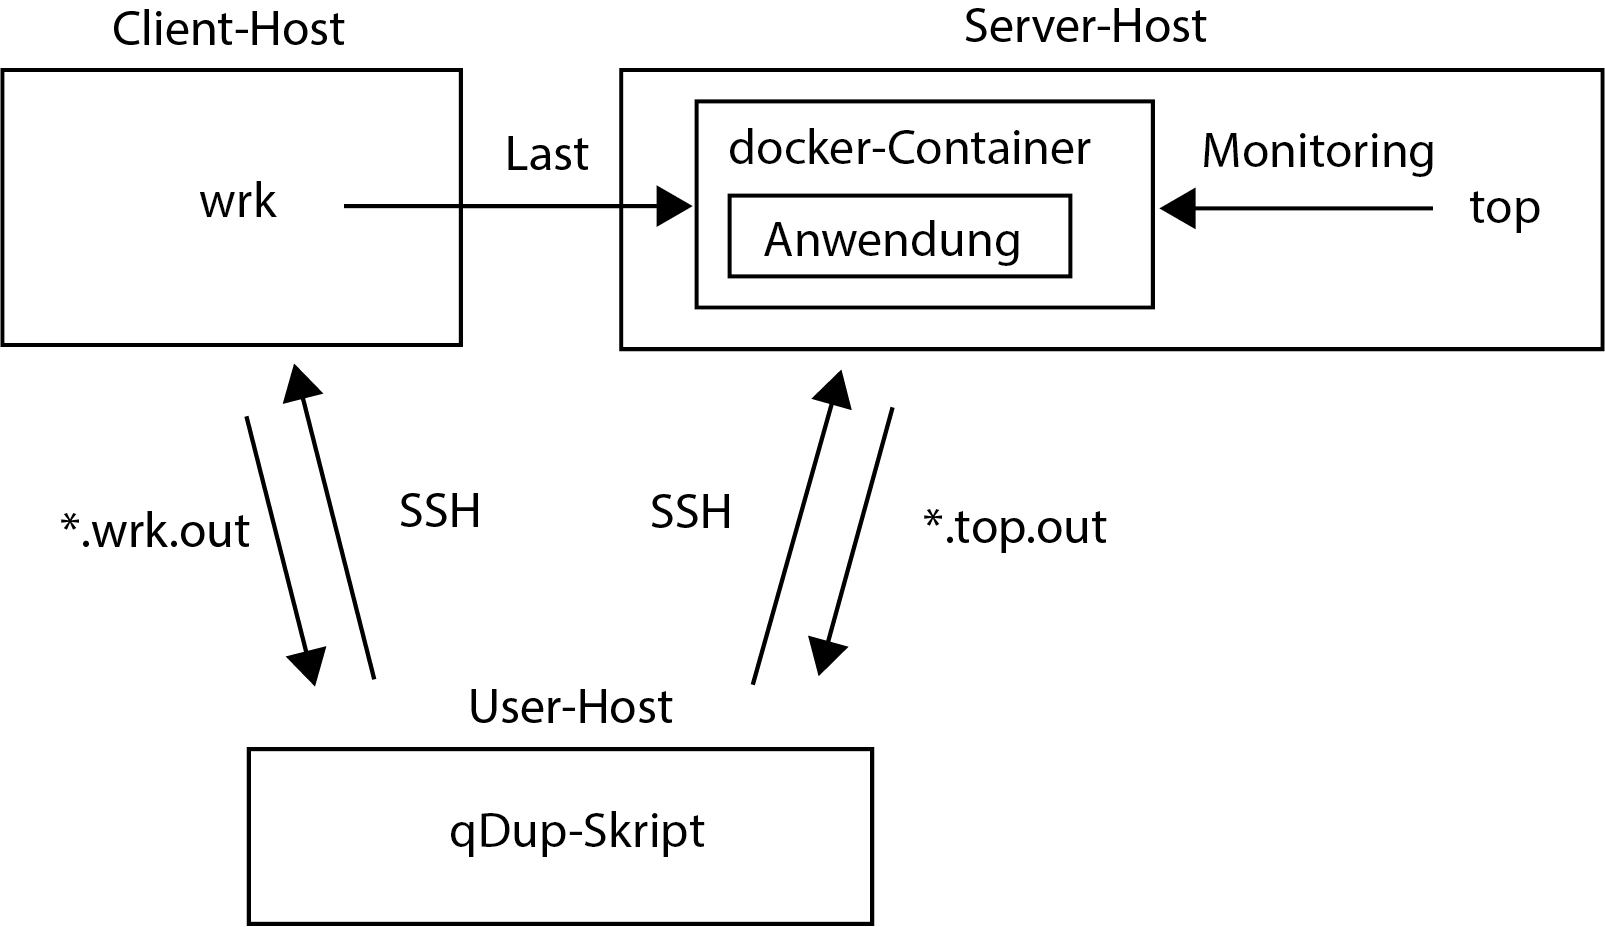
\includegraphics[width=0.8\textwidth]{Testaufbau}
    \caption{Testaufbau}
\end{figure}

In einem Bash-Skript werden anschließend die Ausgaben von \verb|top| und \verb|wrk| für jede einzelne \verb|workload| eines Tests
über ein Java-Skript, das mit dem Tool \textit{JBang} ausgeführt wird \footnote{JBang erlaubt das direkte Ausführen von .java Dateien},
eingelesen, analysiert und jeweils der Durchschnitt, das Minimum und das Maximum des Durchsatzes, Speicherverbrauches und CPU-Auslastung pro Last ermittelt.
Diese werden dann für die visuelle Darstellung in eine \verb|.json|-Datei geschrieben.
Zu guter Letzt werden die aufbereiteten Daten durch die Node.js-Bibliothek \textit{d3node-linechart} als Liniendiagramme visuell dargestellt.

\subsection{Test: Statische Daten}
\label{subsection:statische_daten}
Im Folgenden werden die Testresultate der 2. Testreihe dargestellt, erläutert und anschließend zusammengefasst.
Die Ergebnisse aller Testreihen können im Projektverzeichnis unter \verb|results/data| und \verb|results/graphs| eingesehen werden.
Der Lasttest mit statischen Daten wird ohne Datenbankanbindung durchgeführt und der angesteuerte Endpunkt \verb|/greeting/{name}| gibt bei beiden Anwendungen
jeweils einen statischen String zurück. Wie bereits zu Beginn des Kapitels erwähnt, wird jede Anwendung sowohl im \verb|JVM mode|, als auch im
\verb|native mode| getestet.
Die qDup-Skripte befinden sich im Projektverzeichnis im Verzeichnis \verb|scripts/benchmark-jvm-static.yaml| und
\verb|scripts/benchmark-native-static.yaml|.

\subsubsection{JVM mode}
\label{subsubsec:static_jvm_mode}
Wie aus Listing \ref{lst:starttimes_jvm_static} berechnet werden kann, liegt die durchschnittliche Zeit vom Start der Anwendung bis zur
Bearbeitung der ersten Anfrage ohne Datenbankanbindung bei einer reaktiven Anwendung im \verb|JVM mode| bei 1344.8 ms und bei einer
blockierenden Anwendung bei 1526.6 ms.
\begin{lstlisting}[caption=5 gemessene Startzeiten bis zur Bearbeitung der ersten Anfrage: links ist die reaktive Anwendung und rechts
    die blockierende Anwendung, captionpos=b, label=lst:starttimes_jvm_static]
    1344 ms     1575 ms
    1333 ms     1519 ms
    1324 ms     1546 ms
    1345 ms     1477 ms
    1378 ms     1516 ms
\end{lstlisting}

In Abbildung \ref{fig:jvm_static_mean_response} wird die durchschnittlich gemessene Latenz für jede getestete \verb|workload|,
in diesem Diagramm als Durchsatz beschrieben, dargestellt.
Die höchste getestete \verb|workload| beträgt bei der reaktiven Anwendung \textbf{140.000} Anfragen/Sekunde und bei der
nicht-reaktiven Anwendung \textbf{70.000} Anfragen/Sekunde.

Der maximale serverseitige Durchsatz der nicht-reaktiven Anwendung beträgt ~\textbf{68.000} Anfragen/Sekunde mit einer
Latenz von 60 ms und
die reaktive Anwendung erreicht ~\textbf{134.000} Anfragen/Sekunde bei einer durchschnittlichen Latenz von 95ms.
Bei höheren Lasten steigt die Latenz auf deutlich über eine Sekunde, weswegen der Durchsatz stagniert.

Die reaktive Anwendung erreicht also in der vorliegenden Testumgebung für einen trivialen
Endpunkt mit statischen Daten fast den doppelten Durchsatz.
\newpage
\begin{figure}[ht!]
    \centering
    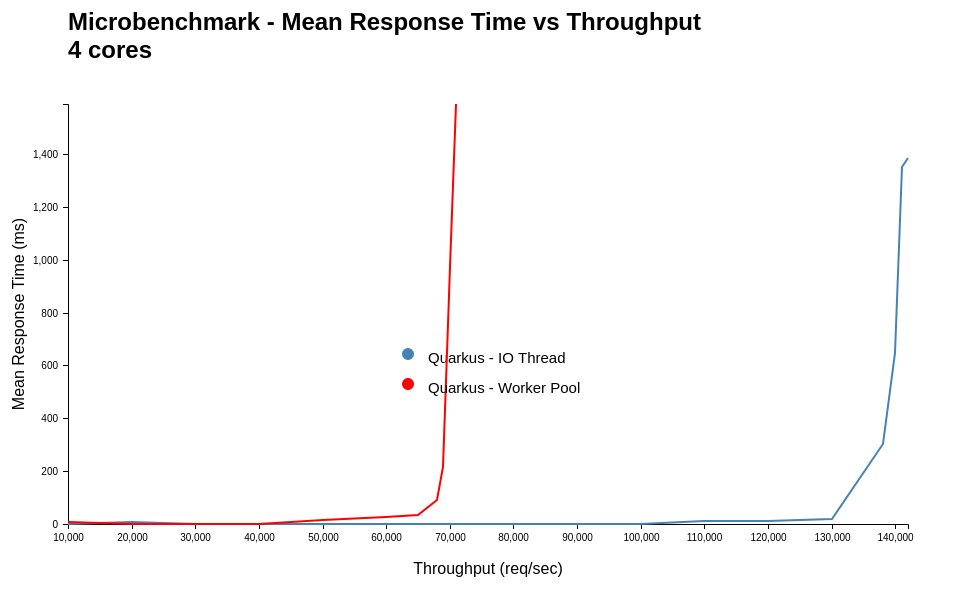
\includegraphics[width=0.9\textwidth]{run2/jvm-static/mean-response-vs-throughput}
    \caption{Test mit statischen Ressourcen im JVM mode: Durchschnittliche Latenz jeder Last}
    \label{fig:jvm_static_mean_response}
\end{figure}

Abbildung \ref{fig:jvm_static_mean_rss} stellt den durchschnittlich allokierten Speicher des jeweiligen Anwendungsprozesses im Hauptspeicher
für jede \verb|workload| dar. Der allokierte Speicher für die genannten maximalen Durchsätze
beträgt dabei bei der reaktiven Anwendung ~\verb|583 MB| und bei der
blockierenden, nicht-reaktiven Anwendung ~\verb|826 MB|.

\begin{figure}[ht!]
    \centering
    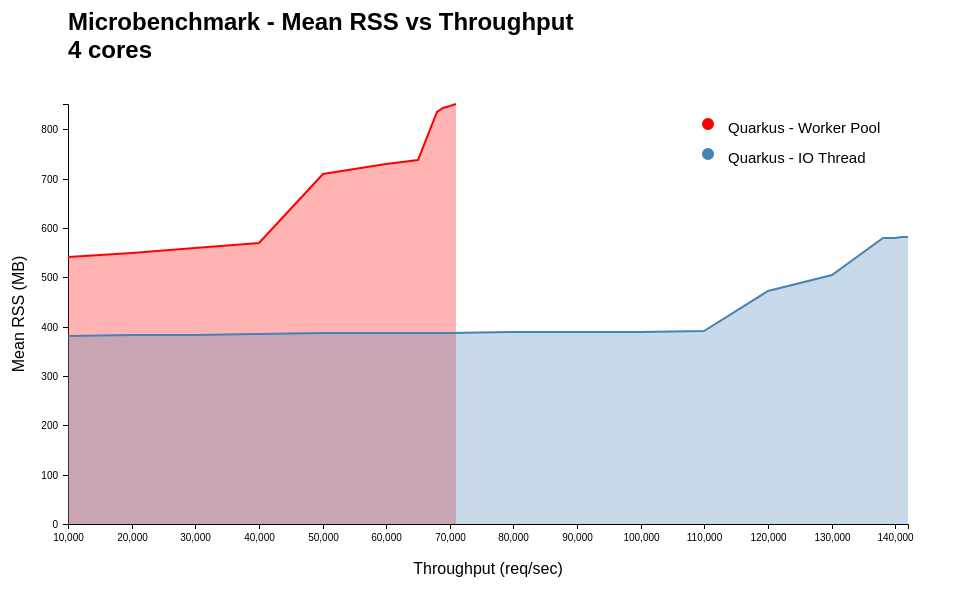
\includegraphics[width=0.9\textwidth]{run2/jvm-static/mean-rss-vs-throughput}
    \caption{Test mit statischen Ressourcen im JVM mode: Allokierter Hauptspeicher pro workload}
    \label{fig:jvm_static_mean_rss}
\end{figure}
\newpage
Zu guter Letzt wird in Abbildung \ref{fig:jvm_static_avg_cpu} die durchschnittlich gemessene CPU-Auslastung für jede \verb|workload| dargestellt.
Bei der nicht-reaktiven Anwendung wird eine durschnittliche CPU-Auslastung von 99\% bereits bei einer Last von 50.000 Anfragen/Sekunde erreicht, die reaktive Anwendung hingegen erreicht diese Auslastung erst bei 120.000 Anfragen/Sekunde.
\begin{figure}[ht!]
    \centering
    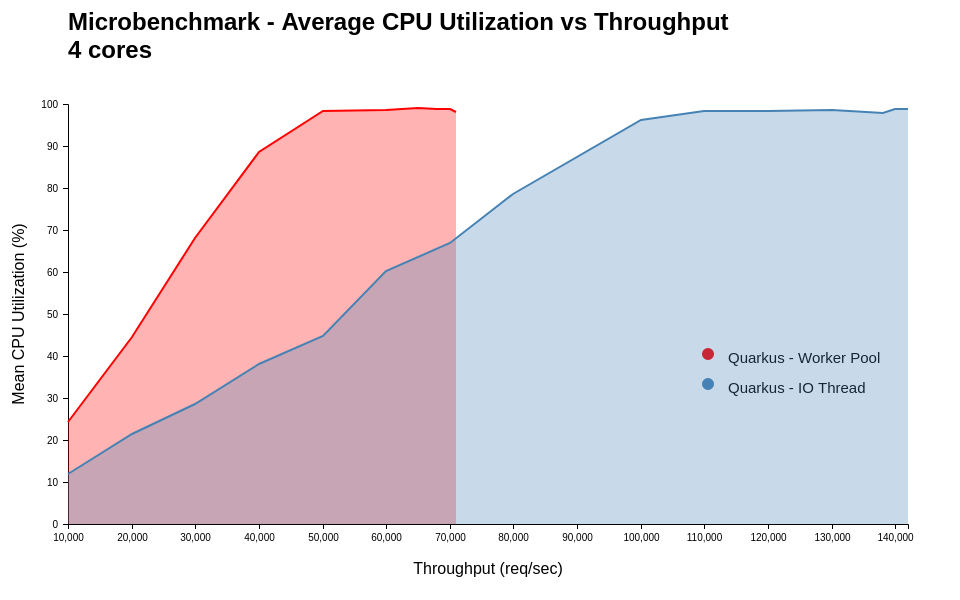
\includegraphics[width=0.9\textwidth]{run2/jvm-static/average-cpu-vs-throughput}
    \caption{Test mit statischen Ressourcen im JVM mode: CPU Auslastung pro workload}
    \label{fig:jvm_static_avg_cpu}
\end{figure}

In Tabelle \ref{table:static_jvm_measurement_results} werden die Resultate der gemessenen Benchmarks zusammengefasst
und zueinander ins Verhältnis gesetzt. Im JVM mode mit statischen Ressourcen erreicht die reaktive Anwendung
eine ~13\% schnellere durchschnittliche Startzeit bis vollständigen Bearbeitung der ersten Anfrage, sowie
einen um ~30\% geringeren Speicherverbrauch.
Darüber hinaus wird ein um etwa 97\% höherer maximaler Durchsatz erzielt, bevor die Latenz eine Sekunde übersteigt, und
es können 140\% mehr Anfragen pro Sekunde verarbeitet werden bis die CPU Auslastung, mit dem in Tabelle \ref{table:system_host}
genannten CPU, bei 4 Kernen 99\% erreicht.

\begin{table}[ht!]
    \begin{tabular}{|l | c | c | c|}
        \hline
        Run 2 - JVM mode - Static - 4 Cores & Blockierend & Reaktiv & Verhältnis \\
        \hline
        \makecell{Durchschn. Startzeit bis erste Anfrage                         \\(ms)} & 1526.6      & 1344.8  & 87,4\%     \\
        \hline
        Max. allokierter RAM (MB)           & 826         & 583     & 70.5\%     \\
        \hline
        Max. Durchsatz (req/sec)            & 68.000      & 134.000 & 197\%      \\
        \hline
        CPU Auslastung bei 99\% (req/sec)   & 50.000      & 120.000 & 240\%      \\
        \hline
    \end{tabular}
    \caption{Verhältnis der gemessenen Benchmarks für beide Anwendungen im JVM mode mit statischen Ressourcen}
    \label{table:static_jvm_measurement_results}
\end{table}

\subsubsection{native mode}
\label{subsubsec:static_native_mode}
Wie aus Listing \ref{lst:starttimes_native_static} berechnet werden kann, liegt die durchschnittliche Zeit vom Start der Anwendung bis zur
Bearbeitung der ersten Anfrage ohne Datenbankanbindung bei einer reaktiven Anwendung im \verb|native mode| bei 28 ms und bei einer
blockierenden Anwendung bei 28.6 ms. Beide Anwendungen benötigen also in etwa die gleiche Zeit.

\begin{lstlisting}[caption=5 gemessene Startzeiten bis zur Bearbeitung der ersten Anfrage: links ist die reaktive Anwendung und rechts
    die blockierende Anwendung, captionpos=b, label=lst:starttimes_native_static]
    28 ms     29 ms
    28 ms     29 ms
    28 ms     29 ms
    28 ms     28 ms
    28 ms     28 ms
\end{lstlisting}

In Abbildung \ref{fig:native_static_mean_response} wird die durchschnittlich gemessene Latenz für jede getestete \verb|workload|,
in diesem Diagramm als Durchsatz beschrieben, dargestellt.
Die höchste getestete \verb|workload| beträgt bei der reaktiven Anwendung \textbf{140.000} Anfragen/Sekunde und bei der
nicht-reaktiven Anwendung \textbf{70.000} Anfragen/Sekunde.

Der maximale serverseitige Durchsatz der nicht-reaktiven Anwendung beträgt ~\textbf{68.000} Anfragen/Sekunde mit einer
Latenz von 60 ms und
die reaktive Anwendung erreicht ~\textbf{134.000} Anfragen/Sekunde bei einer durchschnittlichen Latenz von 95ms.
Bei höheren Lasten steigt die Latenz auf deutlich über eine Sekunde, weswegen der Durchsatz stagniert.

Die reaktive Anwendung erreicht also in der vorliegenden Testumgebung für einen trivialen
Endpunkt mit statischen Daten fast den doppelten Durchsatz.
\begin{figure}[ht!]
    \centering
    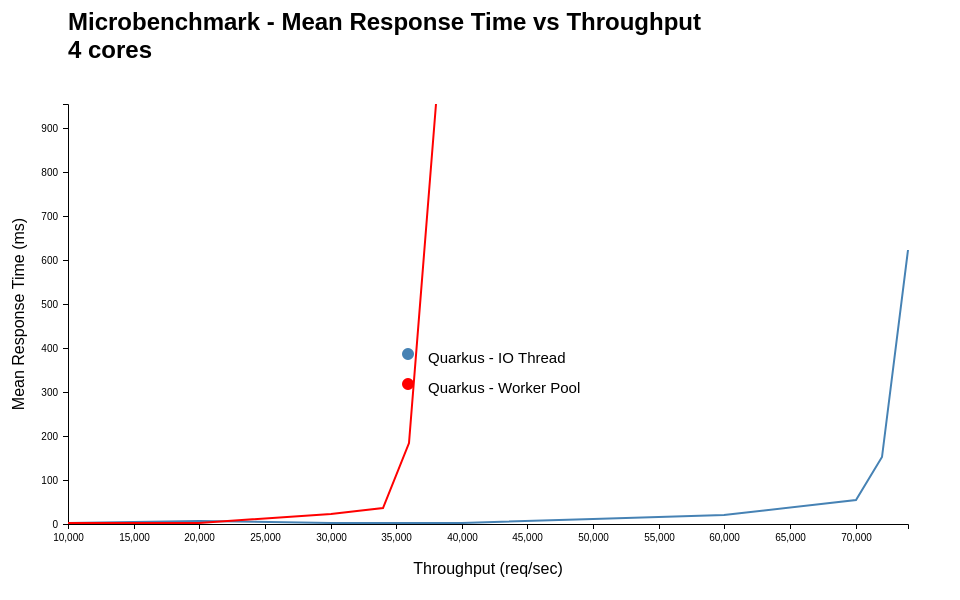
\includegraphics[width=0.9\textwidth]{run2/native-static/mean-response-vs-throughput}
    \caption{Test mit statischen Ressourcen im native mode: Durchschnittliche Latenz jeder Last}
    \label{fig:native_static_mean_response}
\end{figure}

\begin{figure}[ht!]
    \centering
    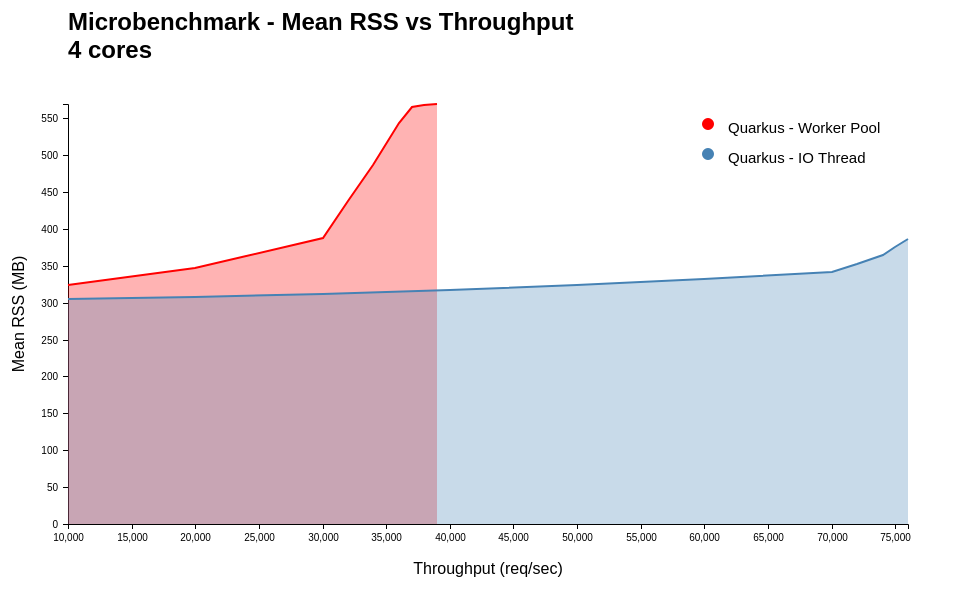
\includegraphics[width=0.9\textwidth]{run2/native-static/mean-rss-vs-throughput}
    \caption{Test mit statischen Ressourcen im native mode: Allokierter Hauptspeicher pro workload}
    \label{fig:native_static_mean_rss}
\end{figure}
\newpage

\begin{figure}[ht!]
    \centering
    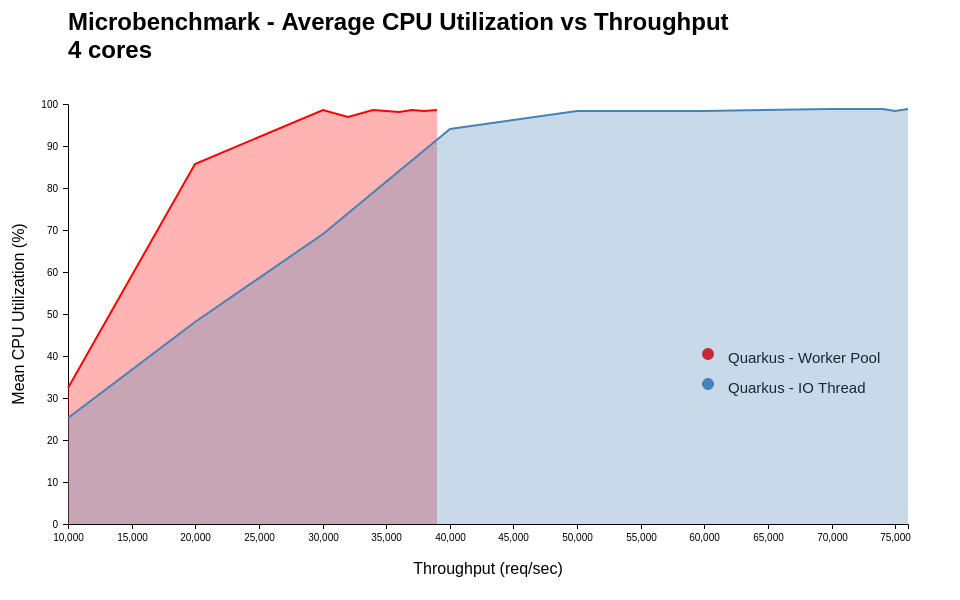
\includegraphics[width=0.9\textwidth]{run2/native-static/average-cpu-vs-throughput}
    \caption{Test mit statischen Ressourcen im native mode: CPU Auslastung pro workload}
    \label{fig:native_static_avg_cpu}
\end{figure}

\begin{table}[ht!]
    \begin{tabular}{|l | c | c | c|}
        \hline
        Run 2 - native mode - Static - 4 Cores & Blockierend & Reaktiv & Verhältnis \\
        \hline
        \makecell{Durchschn. Startzeit bis erste Anfrage                            \\(ms)} &       &   &      \\
        \hline
        Max. allokierter RAM (MB)              &             &         &            \\
        \hline
        Max. Durchsatz (req/sec)               &             &         &            \\
        \hline
        CPU Auslastung bei 99\% (req/sec)      &             &         &            \\
        \hline
    \end{tabular}
    \caption{Verhältnis der gemessenen Benchmarks für beide Anwendungen im native mode mit statischen Ressourcen}
    \label{table:static_native_measurement_results}
\end{table}





\subsection{Test: Datenbankzugriffe}
\label{section:datenbankzugriffe}
Im Folgenden werden die Testresultate der 2. Testreihe dargestellt und erläutert.
Die Ergebnisse der anderen Testreihen können im Projektverzeichnis unter \verb|results/data| und \verb|results/graphs| eingesehen werden.
Der Lasttest mit dynamischen Daten wird mit Datenbankanbindung durchgeführt und der angesteuerte Endpunkt \verb|/fruits| gibt bei beiden Anwendungen
jeweils alle Elemente der Tabelle \textit{fruits} zurück. Wie bereits zu Beginn des Kapitels erwähnt, wird jede Anwendung sowohl im \verb|JVM mode|, als auch im
\verb|native mode| getestet, die qDup-Skripte befinden sich im Projektverzeichnis im Verzeichnis \verb|scripts/benchmark-jvm-db.yaml| und
\verb|scripts/benchmark-native-db.yaml|.

\subsubsection{JVM mode}
\label{subsubsec:dynamic_jvm_mode}

//startzeiten
//Speicherverbrauches
//cpu Auslastung
//durchsatz
\subsubsection{native mode}
\label{subsubsec:dynamic_native_mode}

//startzeiten
//Speicherverbrauches
//cpu Auslastung
//durchsatz

\subsection{Auswertung}
\label{subsubsec:auswertung}
//natürlich auch erwähnen das die versuchsreihen leicht varrieren bspw. bei startzeiten der native images
//wie könnte ergebnis aussehen mit komplexeren queries
//ressourcenbedarf von reaktiver anwendung könnte noch weiter gesenkt werden, allerdings wird der worker thread pool von vert.x aus
kompatibilätsgründen zu blocking i/o genutzt
//native anwendungen starten gleichschnell etc. unabhängig von der anwendungsarchitektur
//native anwendungen können (noch) nicht den durchsatz von jvm anwendungen erreichen (ist aber theoretisch laut entwicklern möglich), da
viele laufzeit optimierungen wegfallen
//in startzeiten und ressourcenverbrauch native anwendungen allerdings überlegen
//reaktive anwendungen lohnen sich erst ab bestimmter req/sec
//könnte verändert werden durch: bessere hardware, anpassen der worker thread pool größe und event loop thread pool größe
//,weglassen von vert.x für den test der blockierenden anwendung da dispatching von io thread auf blocking thread auch kosten verursacht, Quarkus
nutzut allerdings immer vert.x, verändern der gepoolten datenbank verbindungen, komplexere queries (verhältnis der größenordnungen wäre aber gleich)


//eher fazit
und erfordern das alle komponenten reaktiv sind (also auch alle library hesteller)
//lösungen wie project loom deutlich komfortabler in  zukunft
\label{section:auswertung}
\section{Fazit}
\label{sec:fazit}

\subsection{Zusammenfassung}
\label{subsec:zusammenfassung}
Ziel der Masterarbeit war es zu untersuchen, ob reaktive, auf \verb|Nonblocking I/O| und dem \verb|Multi-Reactor|-Modell basierende,
Anwendungen das Problem der begrenzten Skalierbarkeit von nicht-reaktiven, auf \verb|Blocking I/O| und dem \verb|Thread per Request|
-Modell basierenden Anwendungen durch Vermeidung von Threadwechseln lösen können, sowie mögliche Alternativen zu beschreiben.

Für diesen Zweck wurden zwei simple Anwendungen als REST-APIs geschrieben, jeweils reaktiv und nicht-reaktiv, deren
performancekritische Metriken durch mehrere Reihen von Lasttests mit variierenden \verb|workloads| gemessen wurden.
Diese Metriken sind die CPU-Auslastung, der Speicherverbrauch, die Startzeit bis zur Bearbeitung der ersten Anfrage,
sowie der Durchsatz und die durchschnittliche Latenz.
Die Anwendungen wurden sowohl im \verb|JVM mode| als auch im \verb|native mode| jeweils mit statischen Ressourcen und dynamischen
Ressourcen, also einer Datenbankanbindung, getestet.
Anschließend wurden die resultierenden Benchmarks der beiden Anwendungen im jeweiligen Modi und Ressourcentyp ausgewertet und
miteinander verglichen.
\newline
Zusammenfassend lassen sich folgende Ergebnisse nennen:\newline

Generell benötigen die \verb|native images| zum Starten nur wenige Millisekunden, was nur ein Bruchteil der Startzeit
von \verb|JVM|-Anwendungen darstellt und allokieren weniger Speicher. Allerdings können Sie nur einen deutlich
geringeren maximalen Durchsatz aufweisen, da auf eine Vielzahl an Laufzeitoptimierungen verzichtet wird.
Sowohl für statische, als auch für dynamische Daten beträgt der maximale Durchsatz der Anwendungen im \verb|native mode|
daher nur circa die Hälfte der Anwendungen im \verb|JVM mode|.

Im \verb|JVM mode| für statische Daten ist die reaktive Anwendung in jeder Metrik überlegen und erzielt mit 140.000 Anfragen/Sekunde
einen ~102\% höheren maximalen Durchsatz, sowie ~31\% weniger Speicherbedarf, eine ~11\% schnellere Startzeit und kann ~120\%
mehr Anfragen bearbeiten, bevor die CPU-Auslastung maximal wird.

Auch im \verb|JVM mode| für dynamische Daten mit Datenbankanbindung ist die reaktive Anwendung in jeder Metrik überlegen und erzielt
mit 36.000 Anfragen/Sekunde einen ~38\% höheren maximalen Durchsatz, sowie ~24\% weniger Speicherbedarf, eine ~17\% schnellere
Startzeit und kann ~80\% mehr Anfragen bearbeiten, bevor die CPU-Auslastung maximal wird.

Abschließend kann festgestellt werden, dass die vorliegende reaktive Anwendung in jeder gemessenen Metrik bessere Werte als ihr
nicht-reaktives, blockierendes Gegenstück erzielen. Während bei statischen Daten die Durchsatzsteigerung über 100\% beträgt, ist die
Steigerung bei dynamischen Daten mit 38\% deutlich geringer, allerdings ist der maximale Durchsatz bei dynamischen Daten auch
um 104.000 Anfragen/Sekunde geringer als bei statischen Daten. Die Datenbank ist bei den Lasttests der begrenzende Faktor.

Die Nachteile von reaktiven Anwendungen sind allerdings der grundlegend unterschiedliche asynchrone, eventorientierte Programmfluss
und der damit verbundene Refactoring-Aufwand, sowie die schwierige Integration in bestehende Programme.

Wenn darüber hinaus der gesamte Leistungsvorteil von reaktiven Anwendungen ausgeschöpft werden soll, ist es erforderlich
dass alle Programmschichten reaktiv sind bzw. reaktive Treiber haben, damit keine Dispatching Kosten verursacht und Threadwechsel
verursacht werden.

\subsection{grenzen der arbeit}
\label{subsec:grenzen_der_arbeit}
Eine vollständige Antwort auf die Frage, ob reaktive Anwendungen besser skalieren als nicht-reaktive Anwendungen
mit \verb|Blocking I/O| kann nicht gegeben werden, da die in dieser Arbeit vorliegenden exemplarischen \verb|workloads|, sowie
die Anwendungsarchitektur und die Datenbankkomplexität von realistischen Systemen abweichen, weswegen die gezeigten Benchmarks
wahrscheinlich nicht zu halten wären.
Darüber hinaus werden Komponenten, welche die Performance eines Gesamtsystems erhöhen wie Load Balancer und Cache-Server
nicht berücksichtigt.

An dieser Stelle empfehlen sich weitere Untersuchungen mit definierten, realitätsnäheren Testumgebungen, um die Vorteile
von reaktiven Anwendungen in der Praxis noch besser beurteilen zu können.
Da die Systemarchitekturen und Arbeitsweisen aber bei jedem Unternehmen variieren, ist für eine schlussendliche Beurteilung
eine individuelle Anpassung essentiell.

\subsection{Ausblick}
\label{subsec:ausblick}
//verweis auf project loom und andere lösungen die nicht erfordern dass anderer programmfluss und programmierparadigma
Es sind noch die folgenden Schritte notwendig…

Wünschenswert ist ein Vergleich der Ergebnisse mit …

Eine lohnende Aufgabe für die nahe Zukunft ist …


%Glossar und Acronyme ohne Seitenzahl anzeigen, auf denen die Begriffe auftauchen
\printglossary[nonumberlist]
\printglossary[type=\acronymtype, nonumberlist]

%Literaturverzeichnis in Inhaltsverzeichnis zeigen
\addcontentsline{toc}{section}{Literaturverzeichnis}
\printbibliography
\end{document}